\documentclass[aspectratio=169]{beamer}
\usetheme{Madrid}
\usecolortheme{default}

\usepackage{fontspec}
\usepackage{polyglossia}
\setmainlanguage{english}
\usepackage{graphicx}
\usepackage{amsmath}
\usepackage{booktabs}

\setbeamertemplate{navigation symbols}{}
\setbeamertemplate{footline}[frame number]
\setbeamerfont{footnote}{size=\tiny}

\newcommand{\fuente}[1]{{\footnotesize\textit{Source: #1}}}

\title[Foundations and Introduction to ML]{Foundations and Introduction to\\Machine Learning}
\subtitle{Course material}
\author{Universidad de Salamanca}
\institute{Faculties of Sciences and Chemical Sciences}
\date{\today}

\begin{document}

% ============================================================
\begin{frame}
  \titlepage
\end{frame}

\begin{frame}{Course structure}
  \begin{enumerate}
    \item \textbf{Foundations}
    \begin{itemize}
      \item History and evolution of machine learning
      \item Fundamental concepts
    \end{itemize}
    \item \textbf{Supervised Learning}
    \begin{itemize}
      \item Regression
      \item Classification
    \end{itemize}
    \item \textbf{Unsupervised Learning}
    \begin{itemize}
      \item Clustering
      \item Dimensionality reduction
      \item Anomaly detection
    \end{itemize}
  \end{enumerate}
\end{frame}

% ============================================================
\section{Foundations}
\begin{frame}
  \centering
  {\Huge Section 1}\\[0.5em]
  {\Large Foundations}
\end{frame}

\subsection{1.1 History and evolution}

\begin{frame}{1.1 History and evolution of ML}
  \begin{itemize}
    \item Machine learning represents a \textbf{new programming paradigm}
    \item Instead of writing rules, the machine \textbf{infers them from data}
    \item Three key elements: input data, labels, and a loss function
    \item Its history has not been linear: cycles of enthusiasm and disillusionment
  \end{itemize}
\end{frame}

\begin{frame}{Timeline}
  \footnotesize
  Cycles of ``summer'' (breakthroughs, funding) and ``winter'' (disillusionment, funding cuts).
  \begin{center}
    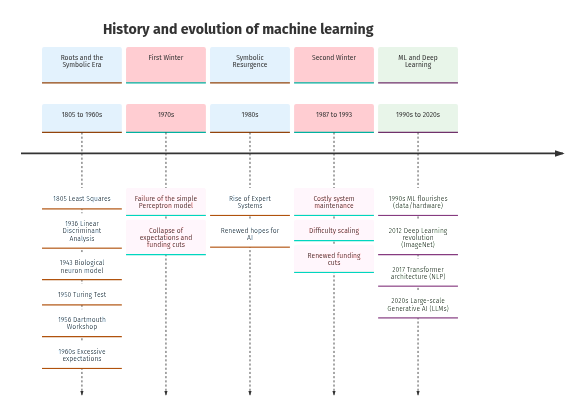
\includegraphics[width=0.62\textwidth]{../book/_static/generated/diagrams_pdf/en/00_fundamentals_01_history_evolution_01.png}
  \end{center}
\end{frame}

\begin{frame}{Mathematical roots and the Turing Test (1805-1950)}
  \begin{columns}
    \begin{column}{0.6\textwidth}
      \begin{itemize}
        \item 1805: Legendre and Gauss, \textbf{least squares}
        \item 1936: Fisher, linear discriminant analysis
        \item 1943: McCulloch and Pitts, first artificial neuron
        \item 1950: Alan Turing, \textit{``Computing Machinery and Intelligence''} — the \textbf{Turing Test}
      \end{itemize}
    \end{column}
    \begin{column}{0.35\textwidth}
      \centering
      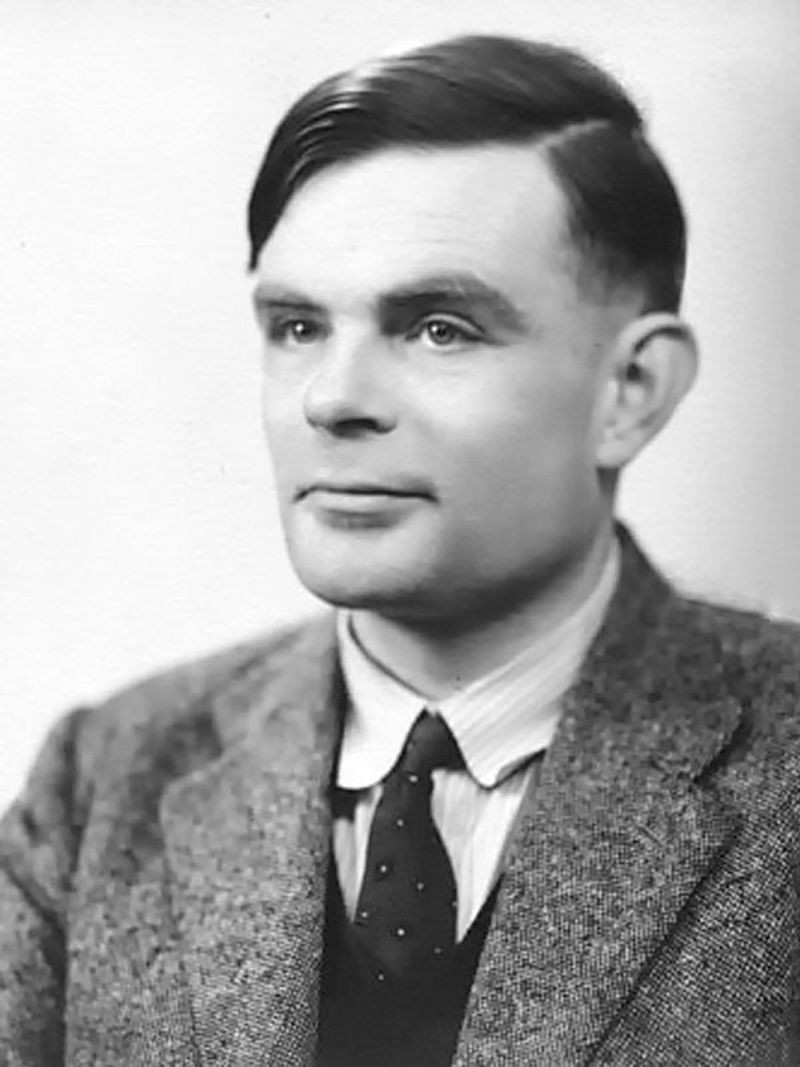
\includegraphics[width=0.85\textwidth]{../book/_static/external_images/alan_turing_1951.jpg}\\[0.3em]
      {\tiny\textit{Source: Elliott \& Fry (1951), public domain}}
    \end{column}
  \end{columns}
\end{frame}

\begin{frame}{The Perceptron and the AI winters}
  \begin{columns}
    \begin{column}{0.6\textwidth}
      \begin{itemize}
        \item 1958: Frank Rosenblatt creates the \textbf{Perceptron}
        \item \textbf{First winter} (1970s): the Perceptron cannot solve non-linear problems
        \item 1956: AI is formally born (Dartmouth workshop)
        \item \textbf{Second winter} (1990s): expert systems prove expensive and hard to scale
      \end{itemize}
    \end{column}
    \begin{column}{0.35\textwidth}
      \centering
      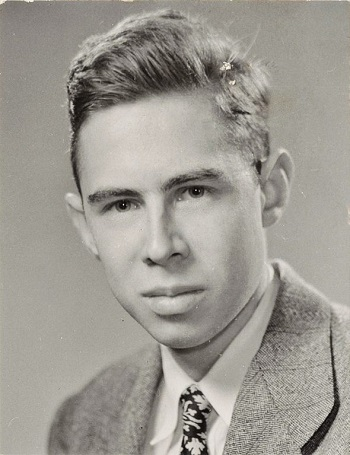
\includegraphics[width=\textwidth]{../book/_static/external_images/frank_rosenblatt.jpg}\\
      \fuente{Heinz Nixdorf MuseumsForum, CC BY-SA 4.0}
    \end{column}
  \end{columns}
\end{frame}

\begin{frame}{Deep Learning and the LLM era (2010-today)}
  \begin{itemize}
    \item 2012: Hinton's victory in the \textbf{ImageNet} challenge
    \item \textbf{MNIST}: the classic benchmark for digit classification
    \item 2017: the \textbf{Transformer} architecture — a revolution in NLP
    \item 2020s: \textbf{Generative AI} (ChatGPT, Gemini) at billion-parameter scale
  \end{itemize}
  \begin{center}
    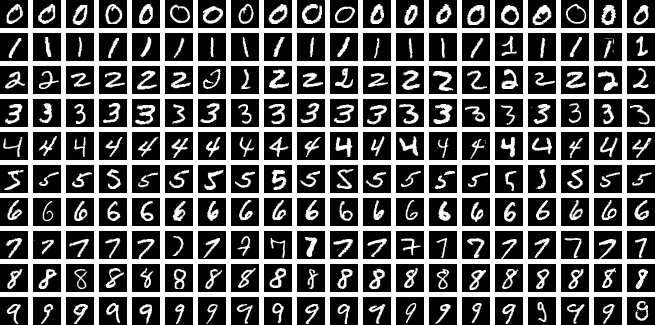
\includegraphics[width=0.55\textwidth]{../book/_static/external_images/mnist_dataset_example.png}\\
    \fuente{Suvanjanprasai (2024), Wikimedia Commons, CC BY-SA 4.0}
  \end{center}
\end{frame}

\subsection{1.2 Fundamental concepts}

\begin{frame}{Data, features, and labels}
  \begin{center}
    \begin{tabular}{lcccc}
      \toprule
      Sample & Feature 1 & Feature 2 & Feature 3 & Label \\
      \midrule
      1 & 25 & 70 & 175 & Cat \\
      2 & 8 & 4 & 90 & Cat \\
      3 & 35 & 80 & 180 & Dog \\
      \bottomrule
    \end{tabular}
  \end{center}
  \vspace{1em}
  \begin{itemize}
    \item \textbf{Sample}: an individual data point
    \item \textbf{Features}: attributes describing the sample
    \item \textbf{Label}: what we want to predict — the ``ground truth''
  \end{itemize}
\end{frame}

\begin{frame}{Overfitting vs. underfitting}
  \begin{itemize}
    \item \textbf{Underfitting}: the model is too simple, misses the pattern (high bias)
    \item \textbf{Overfitting}: the model memorizes training noise (high variance)
    \item Goal: the bias-variance trade-off that generalizes best
  \end{itemize}
  \begin{center}
    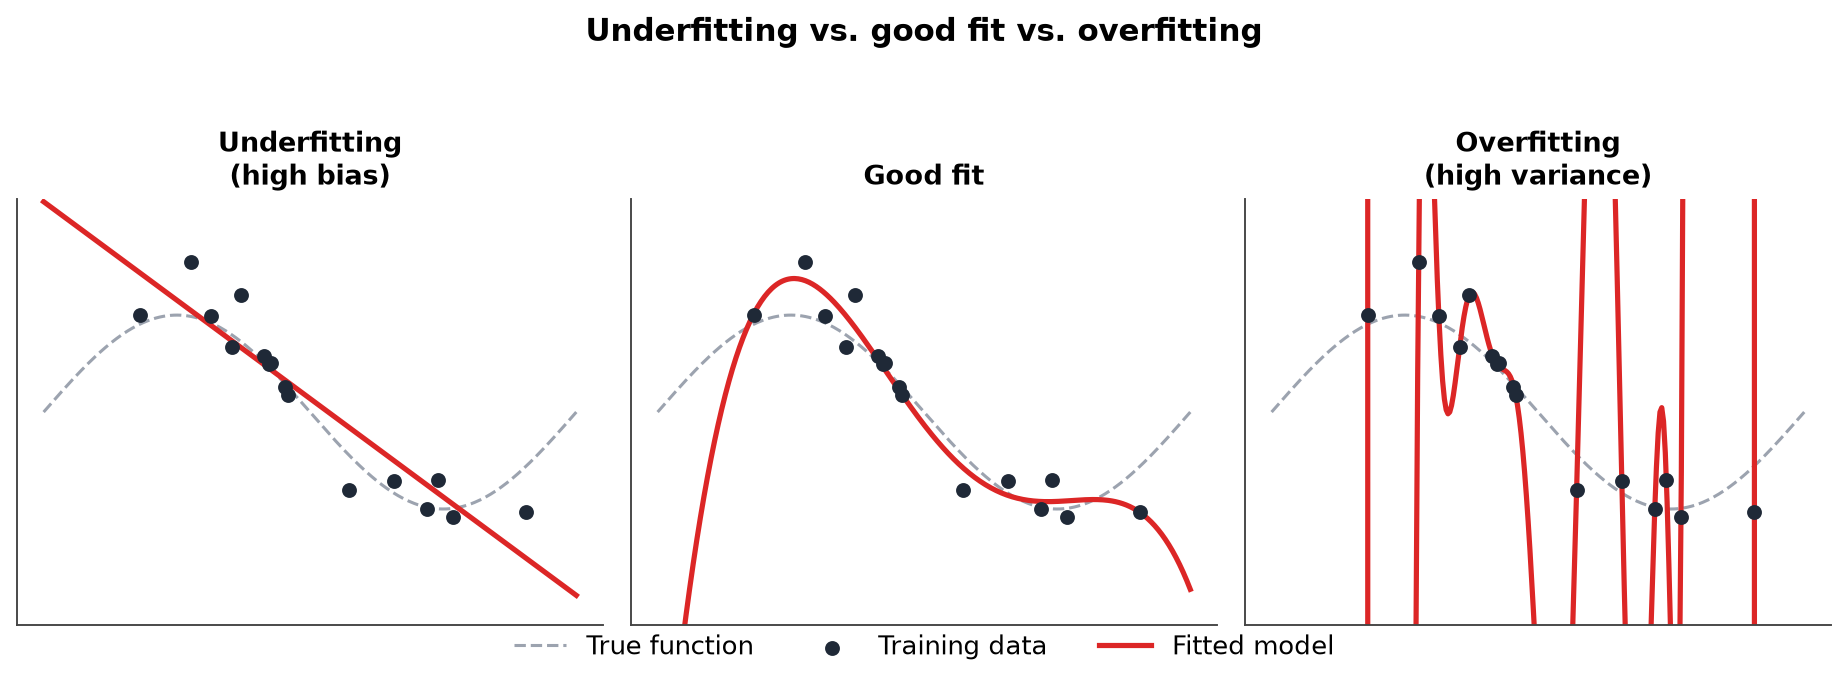
\includegraphics[width=0.75\textwidth]{../book/_static/generated/figures/en/overfitting_underfitting.png}
  \end{center}
\end{frame}

\begin{frame}{$K$-fold cross-validation}
  \begin{itemize}
    \item Splits data into $K$ partitions (\textit{folds}); each one acts once as the test set
    \item Final metric = average of the $K$ results $\rightarrow$ a more robust estimate
    \item Avoids relying on a single train/test split
  \end{itemize}
  \begin{center}
    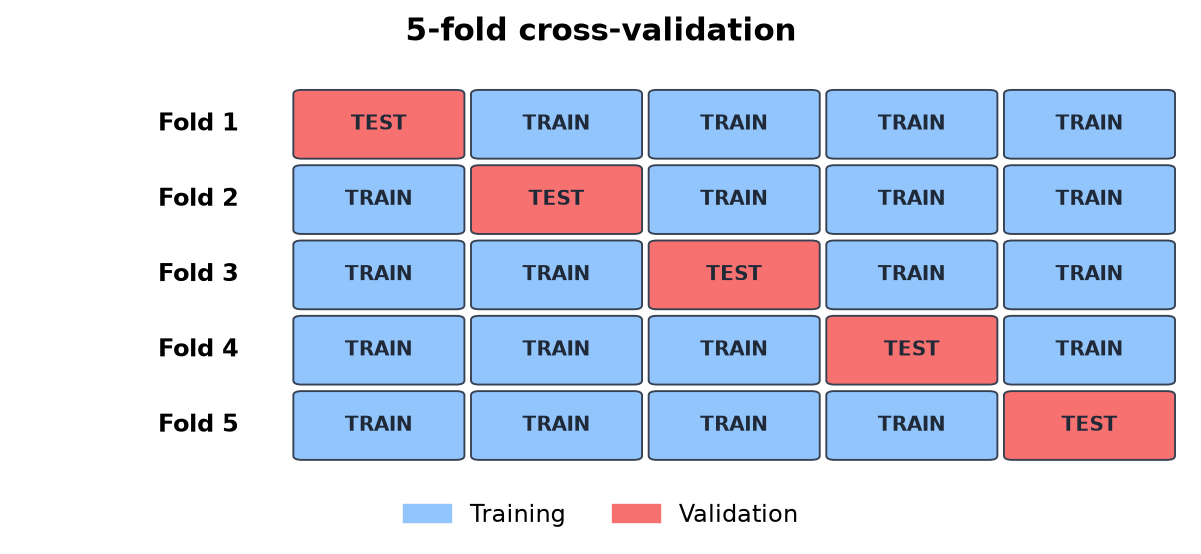
\includegraphics[width=0.62\textwidth]{../book/_static/generated/figures/en/kfold_cross_validation.png}
  \end{center}
\end{frame}

\begin{frame}{Confusion matrix and metrics}
  \begin{columns}
    \begin{column}{0.5\textwidth}
      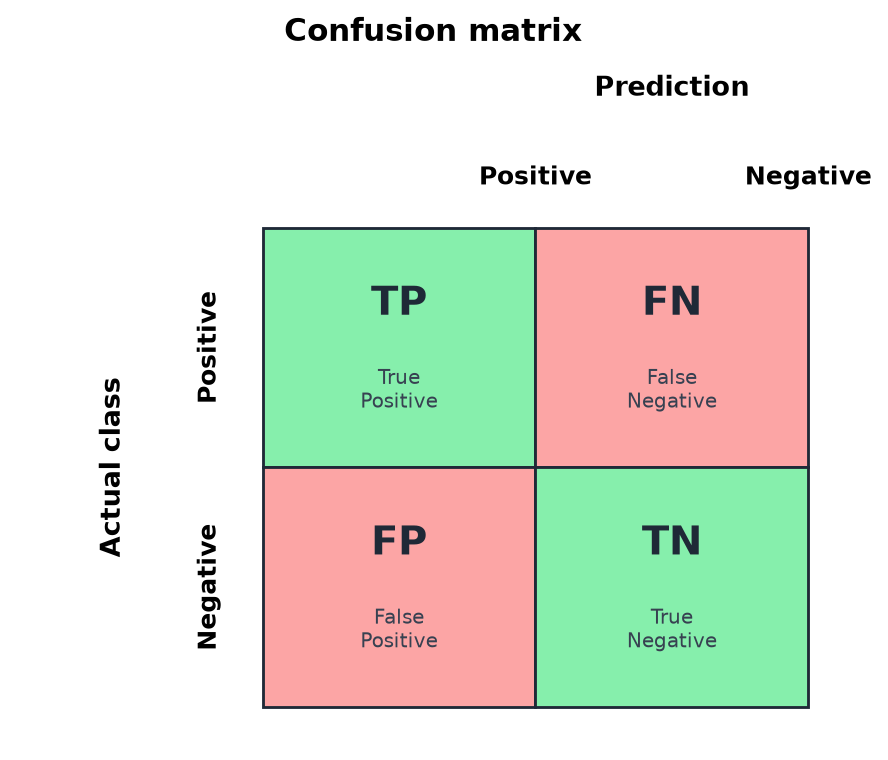
\includegraphics[width=\textwidth]{../book/_static/generated/figures/en/confusion_matrix.png}
    \end{column}
    \begin{column}{0.5\textwidth}
      \small
      \begin{align*}
        \text{Precision} &= \frac{TP}{TP+FP} \\
        \text{Recall} &= \frac{TP}{TP+FN} \\
        F1 &= 2\cdot\frac{P \times R}{P + R}
      \end{align*}
    \end{column}
  \end{columns}
  \vspace{0.5em}
  \footnotesize
  TP/TN: correct predictions; FP/FN: errors. F1 balances precision and recall, useful with imbalanced classes.
\end{frame}

\begin{frame}{The ML \textit{pipeline}: 10 stages}
  \begin{columns}
    \begin{column}{0.42\textwidth}
      \footnotesize
      \begin{itemize}
        \item An \textbf{iterative} process: evaluation can send you back to earlier stages
        \item Much of the real effort lies in stages 2-3 (data) and 7-8 (tuning)
        \item Deployment isn't the end: it requires continuous monitoring
      \end{itemize}
    \end{column}
    \begin{column}{0.55\textwidth}
      \centering
      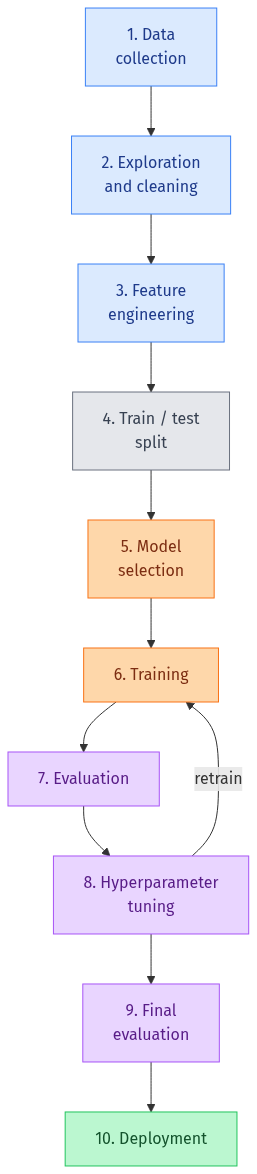
\includegraphics[height=0.8\textheight]{../book/_static/generated/diagrams_pdf/en/00_fundamentals_02_fundamental_concepts_01.png}
    \end{column}
  \end{columns}
\end{frame}

% ============================================================
\section{Supervised Learning}
\begin{frame}
  \centering
  {\Huge Section 2}\\[0.5em]
  {\Large Supervised Learning}
\end{frame}

\subsection{2.1 Regression}

\begin{frame}{Linear regression}
  \begin{itemize}
    \item Predicts a \textbf{continuous value} $Y$ from predictors $X$
    \item Simple: $Y \approx \beta_0 + \beta_1 X$
    \item Multiple: $Y = \beta_0 + \beta_1X_1 + \dots + \beta_pX_p + \epsilon$
    \item \textbf{OLS}: minimizes the residual sum of squares (RSS)
  \end{itemize}
\end{frame}

\begin{frame}{Real example: the \textit{Advertising} dataset}
  \begin{itemize}
    \item Predicts \textit{Sales} from TV, radio, and newspaper advertising spend
    \item The line minimizes the sum of squared residuals (OLS)
    \item Classic example of simple linear regression
  \end{itemize}
  \begin{center}
    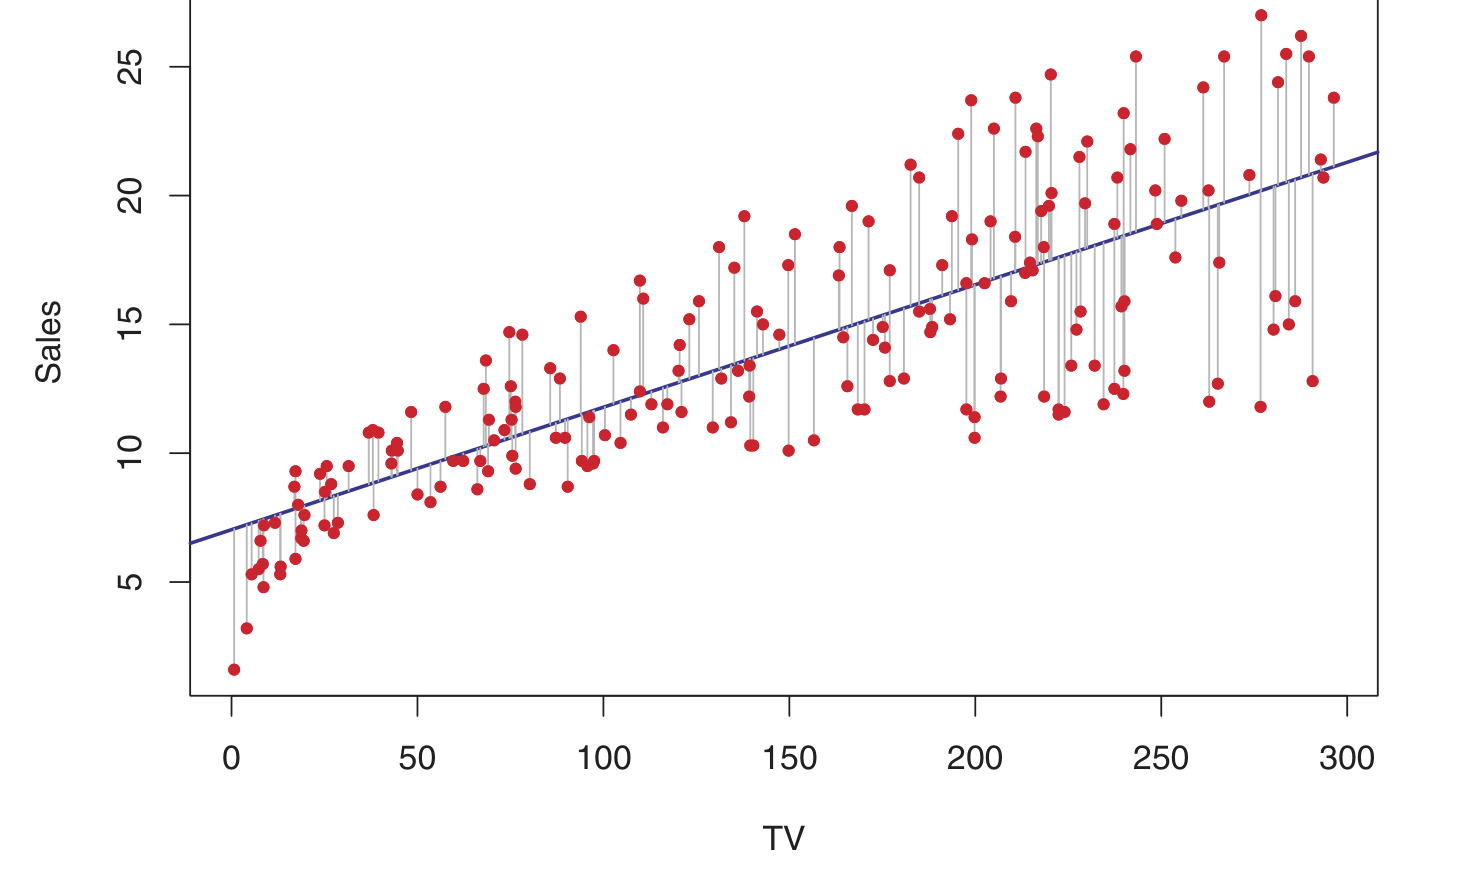
\includegraphics[width=0.48\textwidth]{../book/_static/book_figures/islr_fig3_1_advertising.png}
  \end{center}
  \fuente{James, Witten, Hastie \& Tibshirani (2013), \textit{An Introduction to Statistical Learning}, Fig. 3.1. Freely distributed textbook (statlearning.com).}
\end{frame}

\begin{frame}{Gradient descent}
  \begin{itemize}
    \item Iterative algorithm: updates parameters opposite to the gradient direction
    \item $\theta \leftarrow \theta - \alpha \nabla J(\theta)$, where $\alpha$ is the learning rate
    \item Too high a rate diverges; too low converges slowly
  \end{itemize}
  \begin{center}
    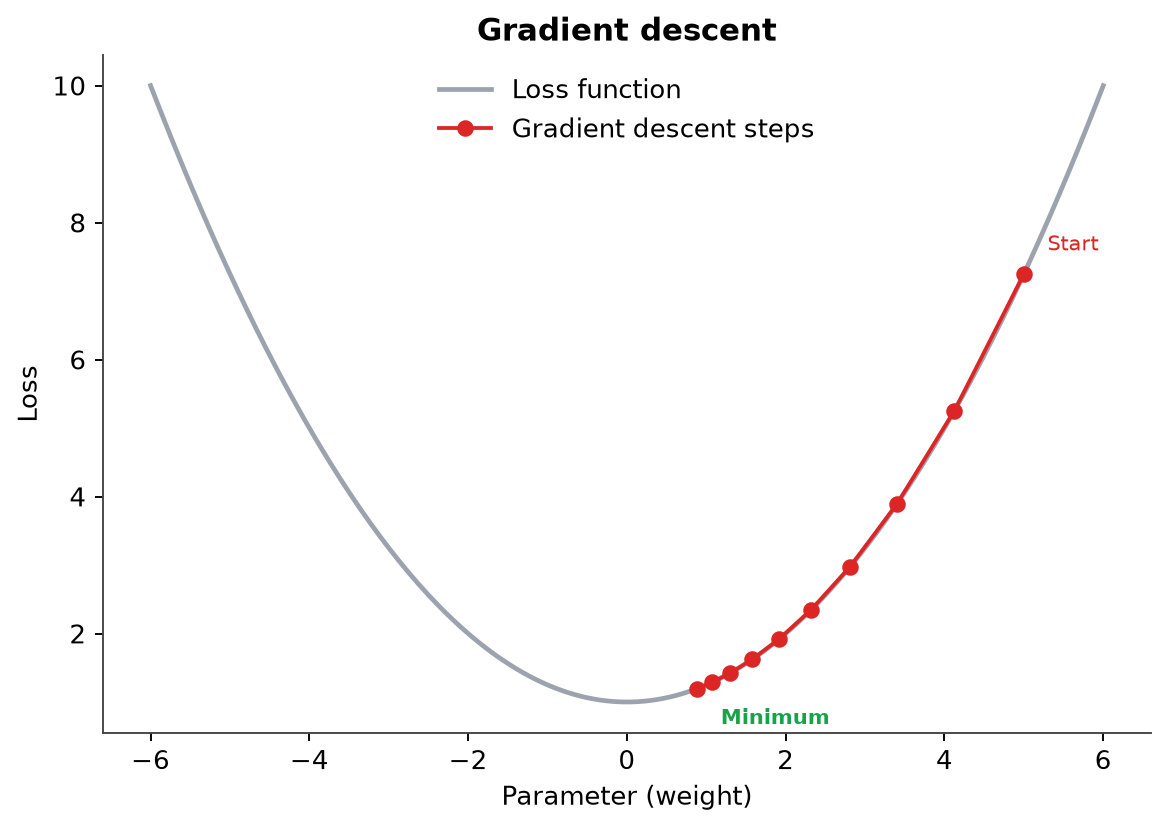
\includegraphics[width=0.5\textwidth]{../book/_static/generated/figures/en/gradient_descent.png}
  \end{center}
\end{frame}

\begin{frame}{Regularization: Ridge and Lasso}
  \begin{itemize}
    \item \textbf{Ridge} ($L_2$): penalizes $\sum \beta_j^2$, shrinks coefficients without zeroing them
    \item \textbf{Lasso} ($L_1$): penalizes $\sum |\beta_j|$, can zero out coefficients (variable selection)
    \item $\lambda$ controls the strength of the penalty
  \end{itemize}
  \begin{center}
    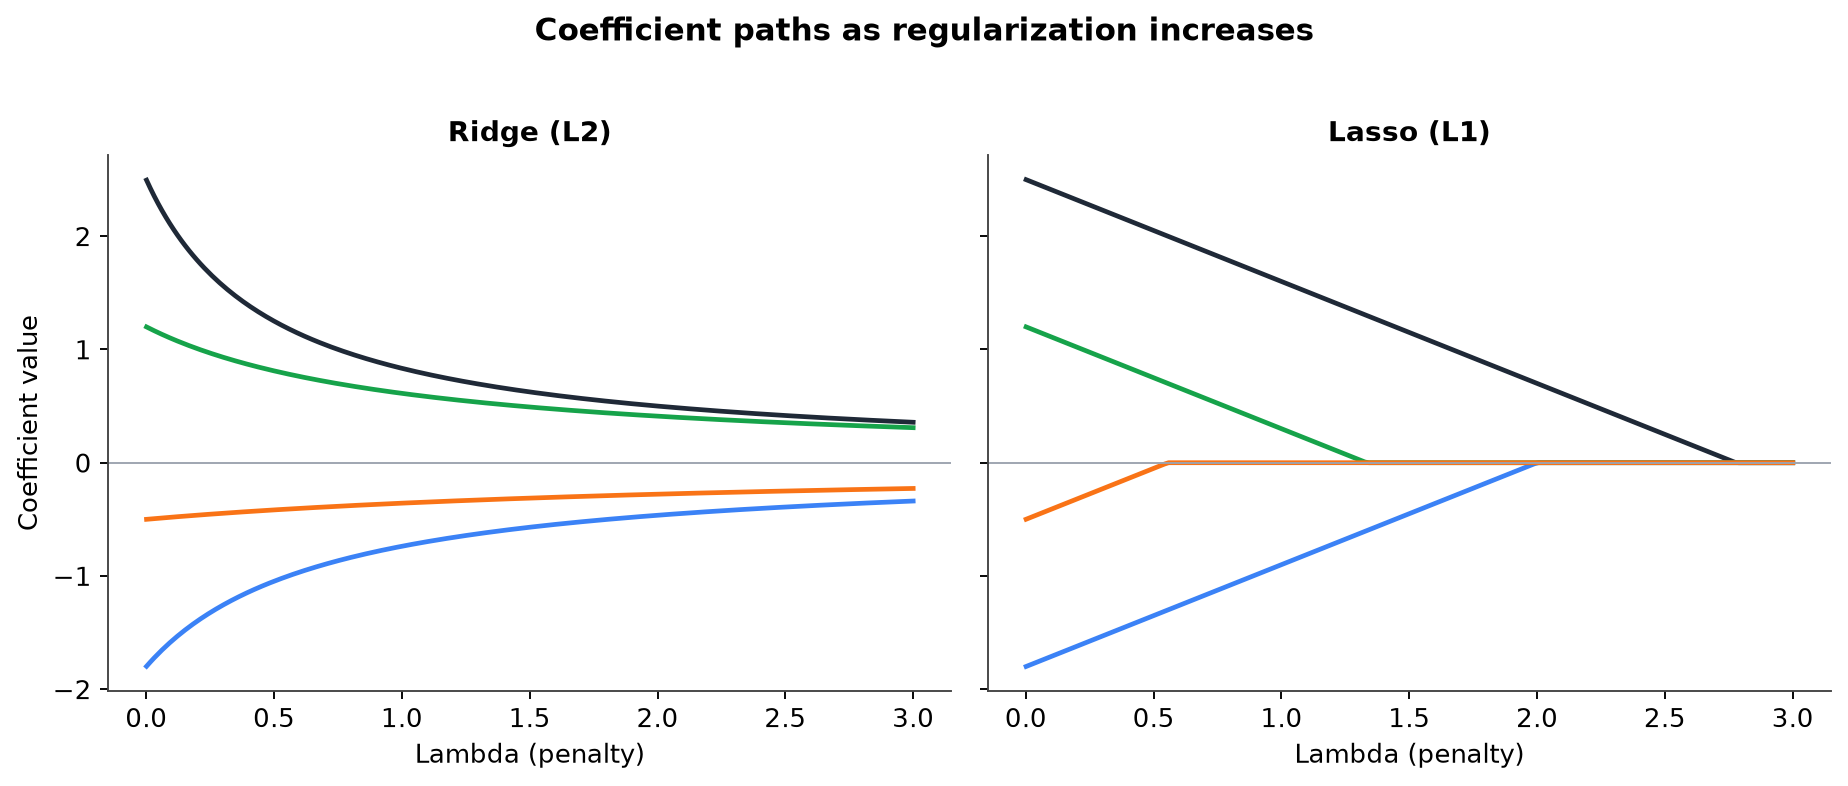
\includegraphics[width=0.7\textwidth]{../book/_static/generated/figures/en/regularization_paths.png}
  \end{center}
\end{frame}

\begin{frame}{Ridge on real data: the \textit{Credit} dataset}
  \begin{itemize}
    \item As $\lambda$ increases, coefficients shrink toward zero
    \item Trades a small increase in bias for a reduction in variance
  \end{itemize}
  \begin{center}
    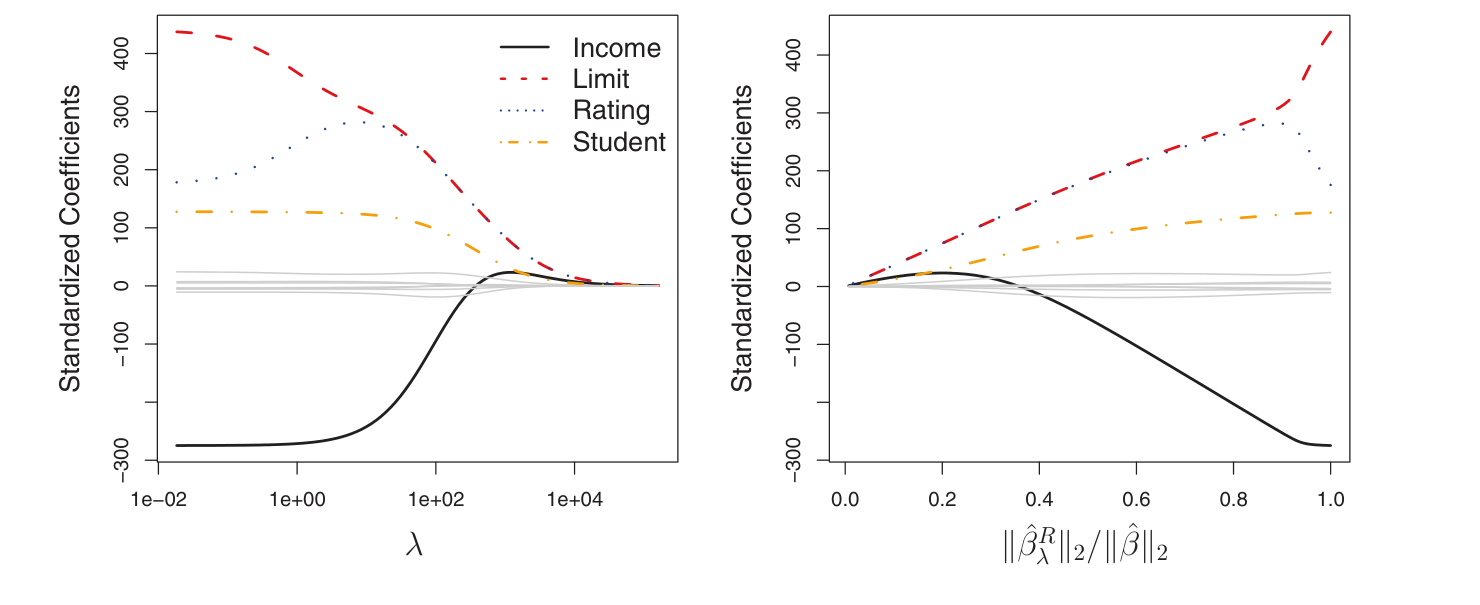
\includegraphics[width=0.65\textwidth]{../book/_static/book_figures/islr_fig6_4_ridge_credit.png}
  \end{center}
  \fuente{James, Witten, Hastie \& Tibshirani (2013), \textit{An Introduction to Statistical Learning}, Fig. 6.4.}
\end{frame}

\subsection{2.2 Classification}

\begin{frame}{The sigmoid function}
  \begin{itemize}
    \item Maps any real value to a probability between 0 and 1
    \item $\sigma(z) = \dfrac{1}{1+e^{-z}}$
    \item The basis of logistic regression
  \end{itemize}
  \begin{center}
    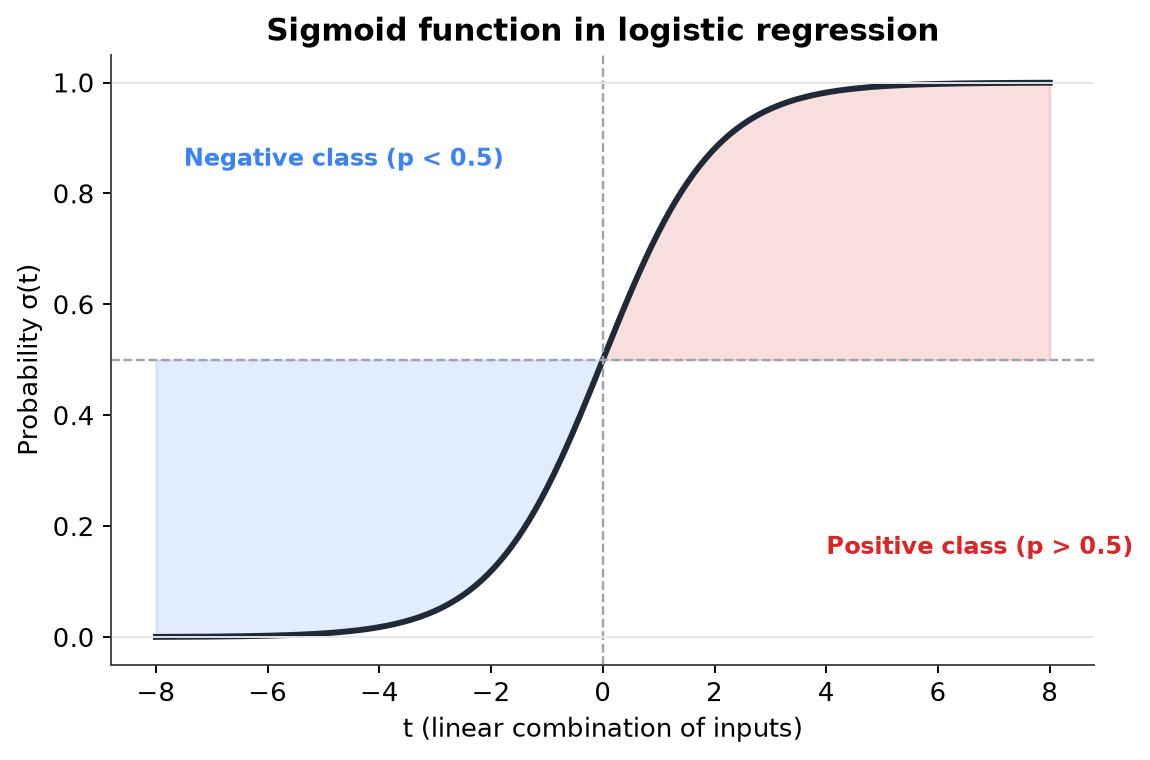
\includegraphics[width=0.5\textwidth]{../book/_static/generated/figures/en/sigmoid_function.png}
  \end{center}
\end{frame}

\begin{frame}{Why not use linear regression?}
  \begin{itemize}
    \item Linear regression can predict probabilities $<0$ or $>1$ (nonsensical)
    \item Logistic regression uses the sigmoid to keep output within $[0,1]$
  \end{itemize}
  \begin{center}
    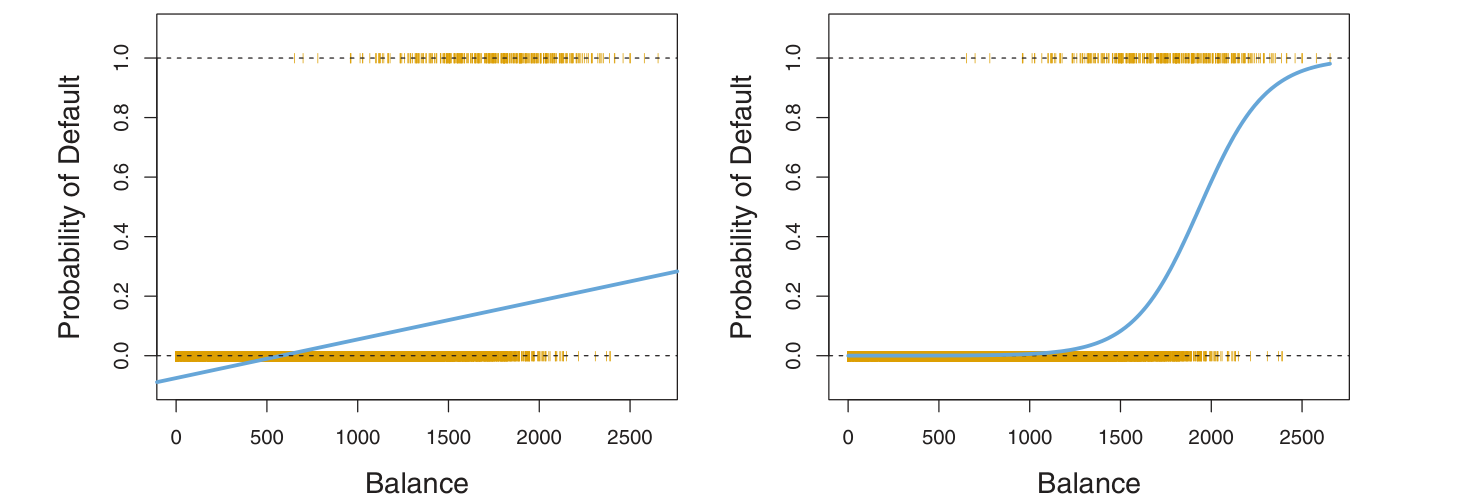
\includegraphics[width=0.7\textwidth]{../book/_static/book_figures/islr_fig4_2_default_logistic.png}
  \end{center}
  \fuente{James, Witten, Hastie \& Tibshirani (2013), \textit{An Introduction to Statistical Learning}, Fig. 4.2.}
\end{frame}

\begin{frame}{Decision trees}
  \begin{columns}
    \begin{column}{0.45\textwidth}
      \begin{itemize}
        \item Splits feature space with successive orthogonal cuts
        \item Each split minimizes child-node impurity (Gini or entropy)
        \item Easy to interpret, but prone to overfitting without pruning
      \end{itemize}
    \end{column}
    \begin{column}{0.5\textwidth}
      \centering
      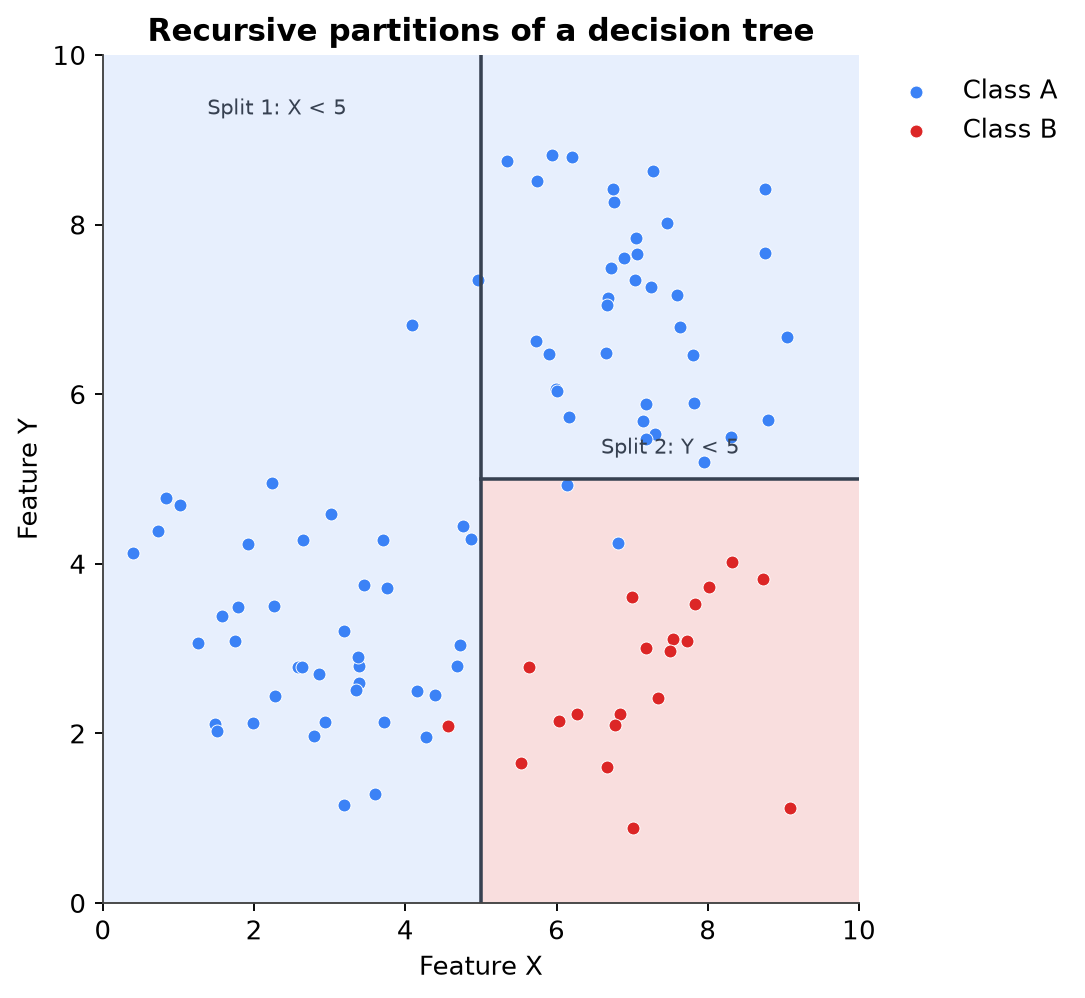
\includegraphics[width=\textwidth]{../book/_static/generated/figures/en/decision_tree_partition.png}
    \end{column}
  \end{columns}
\end{frame}

\begin{frame}{Ensembles: Random Forest and Boosting}
  \begin{itemize}
    \item \textbf{Random Forest}: \textit{bagging} + random feature subset at each split
    \item \textbf{Boosting}: sequential models that correct the previous one's errors (XGBoost, LightGBM)
    \item \textbf{Voting / Stacking}: combine the outputs of several independent models
  \end{itemize}
\end{frame}

\begin{frame}{SVM: maximum margin}
  \begin{columns}
    \begin{column}{0.45\textwidth}
      \begin{itemize}
        \item Finds the hyperplane that maximizes the margin between classes
        \item Support vectors are the points closest to the hyperplane
        \item The \textit{kernel trick} enables non-linear boundaries
      \end{itemize}
    \end{column}
    \begin{column}{0.5\textwidth}
      \centering
      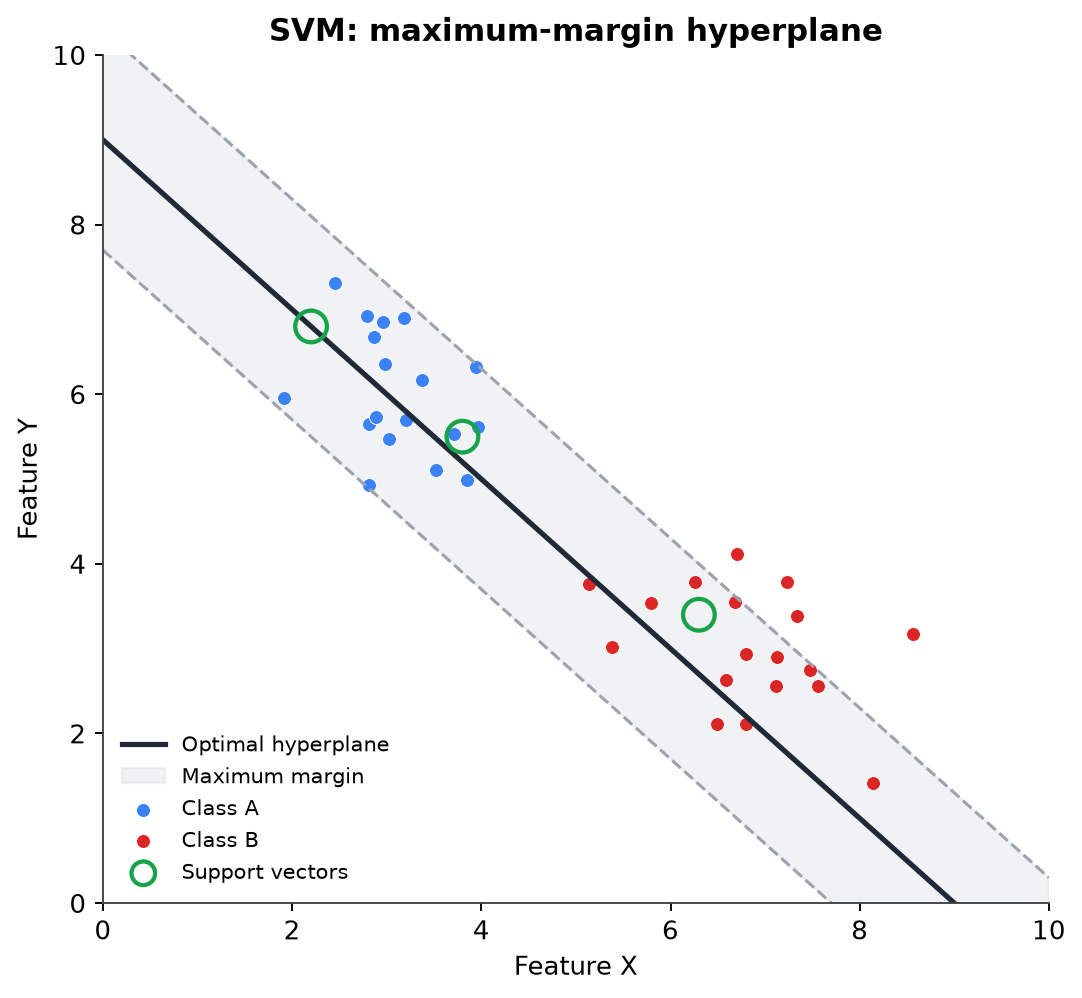
\includegraphics[width=\textwidth]{../book/_static/generated/figures/en/svm_margin.png}
    \end{column}
  \end{columns}
\end{frame}

\begin{frame}{Neural networks}
  \begin{itemize}
    \item Layers of neurons connected by adjustable weights
    \item Each neuron applies a non-linear activation function (ReLU, sigmoid...)
    \item Trained via backpropagation of the error
  \end{itemize}
  \begin{center}
    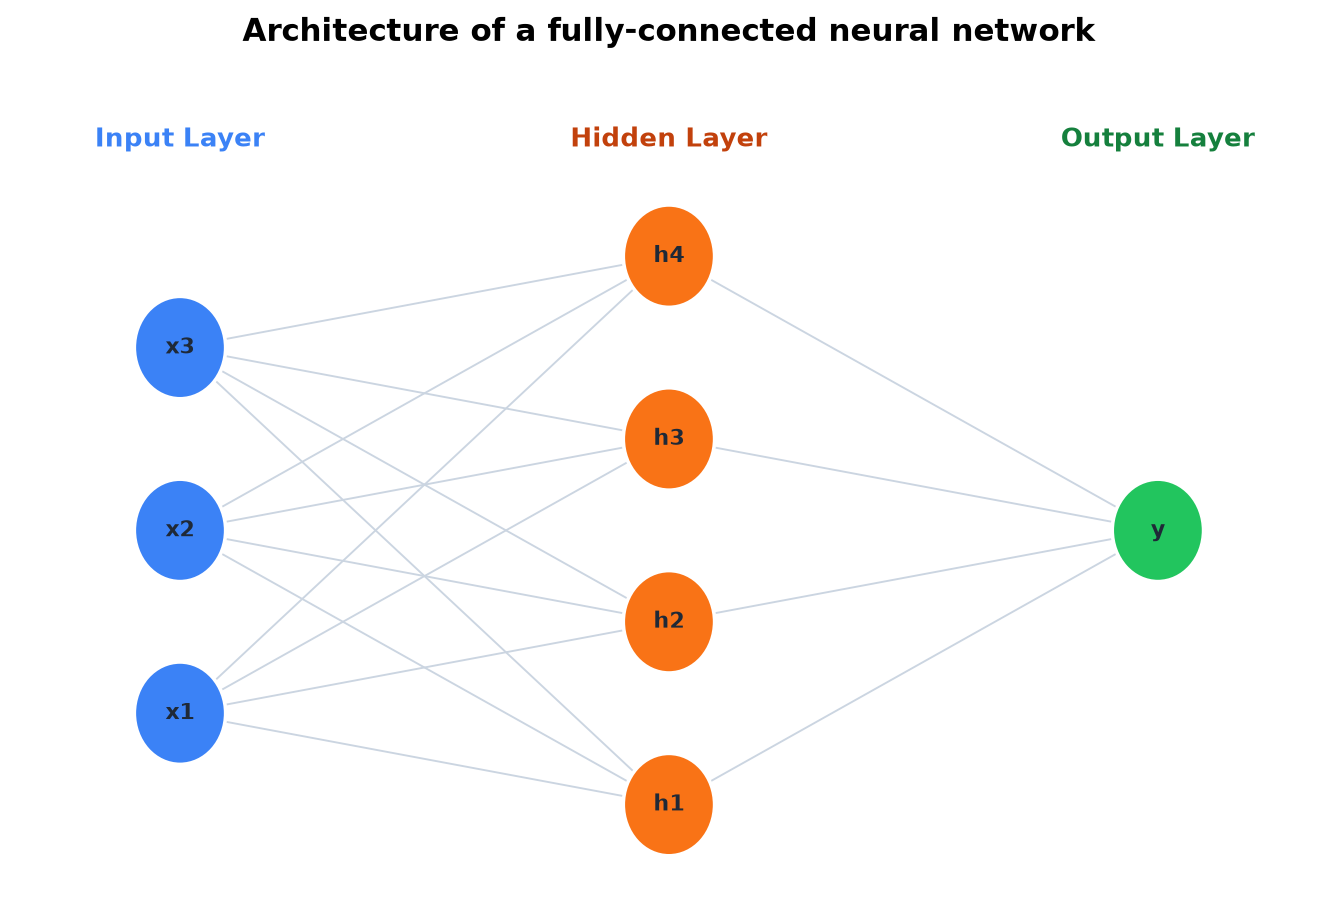
\includegraphics[width=0.5\textwidth]{../book/_static/generated/figures/en/nn_architecture.png}
  \end{center}
\end{frame}

\begin{frame}{Evaluation: ROC curve and AUC}
  \begin{columns}
    \begin{column}{0.45\textwidth}
      \begin{itemize}
        \item Y-axis: true positive rate; X-axis: false positive rate
        \item AUC = 1: perfect classifier; AUC = 0.5: equivalent to random guessing
        \item Compares models independently of the chosen threshold
      \end{itemize}
    \end{column}
    \begin{column}{0.45\textwidth}
      \centering
      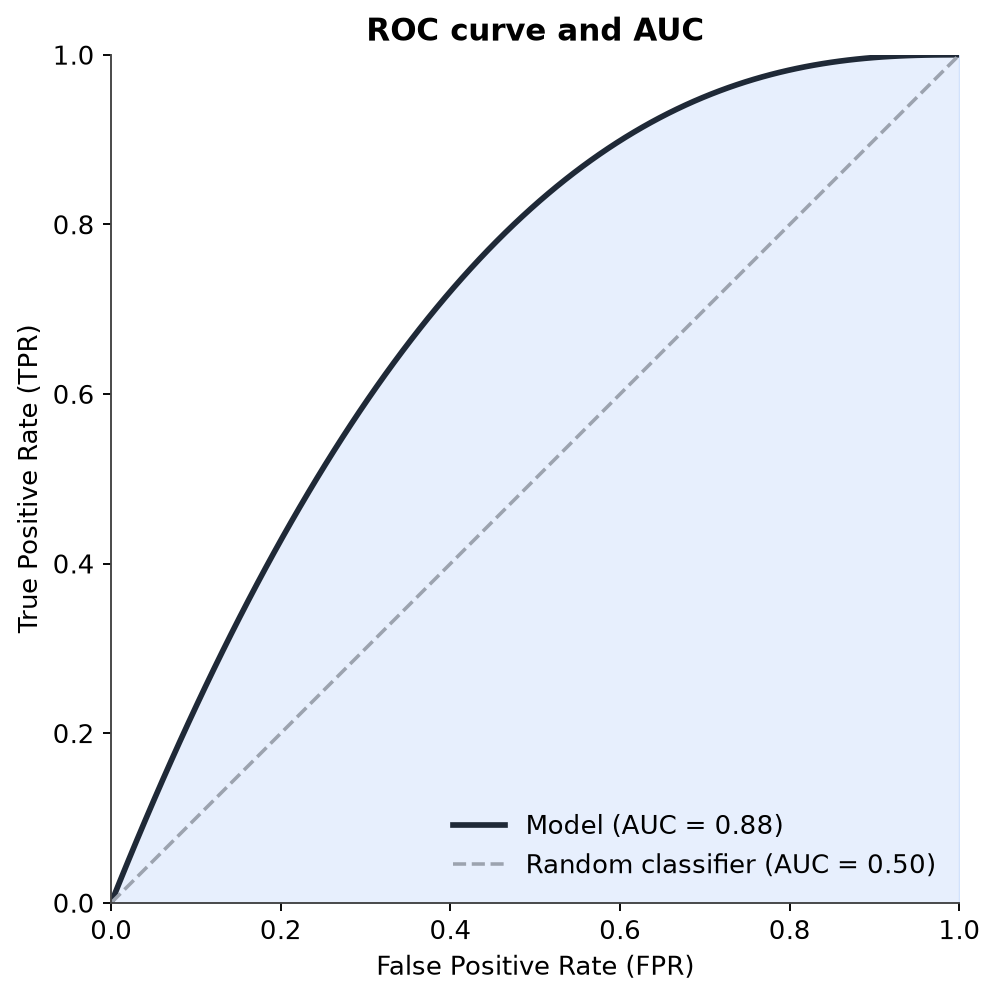
\includegraphics[width=0.9\textwidth]{../book/_static/generated/figures/en/roc_curve.png}
    \end{column}
  \end{columns}
\end{frame}

% ============================================================
\section{Unsupervised Learning}
\begin{frame}
  \centering
  {\Huge Section 3}\\[0.5em]
  {\Large Unsupervised Learning}
\end{frame}

\subsection{3.1 Clustering}

\begin{frame}{What is clustering?}
  \begin{itemize}
    \item No labels: we only have $X$, no $y$
    \item Goal: group data with \textbf{high internal similarity} and \textbf{high external differentiation}
    \item Algorithms: $K$-means, hierarchical, DBSCAN
  \end{itemize}
\end{frame}

\begin{frame}{The iterative $K$-means process}
  \footnotesize
  \begin{enumerate}
    \item Initialize $K$ centroids randomly
    \item Assign each point to the nearest centroid
    \item Recompute centroids as the mean of their cluster; repeat until convergence
  \end{enumerate}
  \begin{center}
    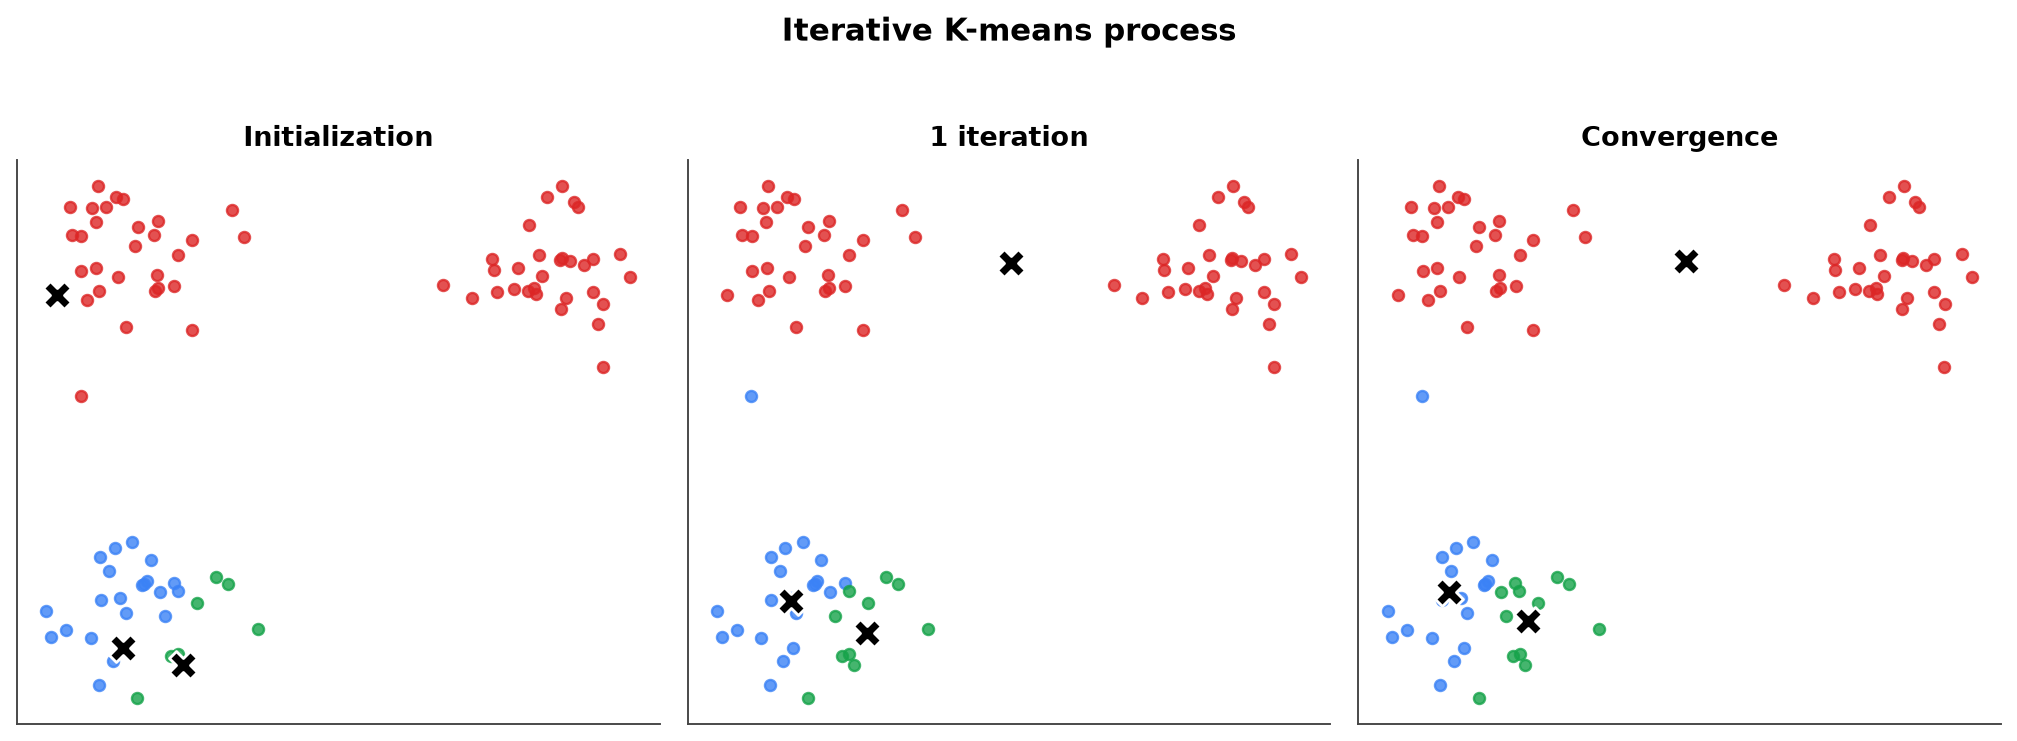
\includegraphics[width=0.85\textwidth]{../book/_static/generated/figures/en/kmeans_process.png}
  \end{center}
\end{frame}

\begin{frame}{The elbow method}
  \begin{itemize}
    \item Plots inertia (sum of squared distances) against $K$
    \item The ``elbow'' marks the point of diminishing returns: the optimal $K$
  \end{itemize}
  \begin{center}
    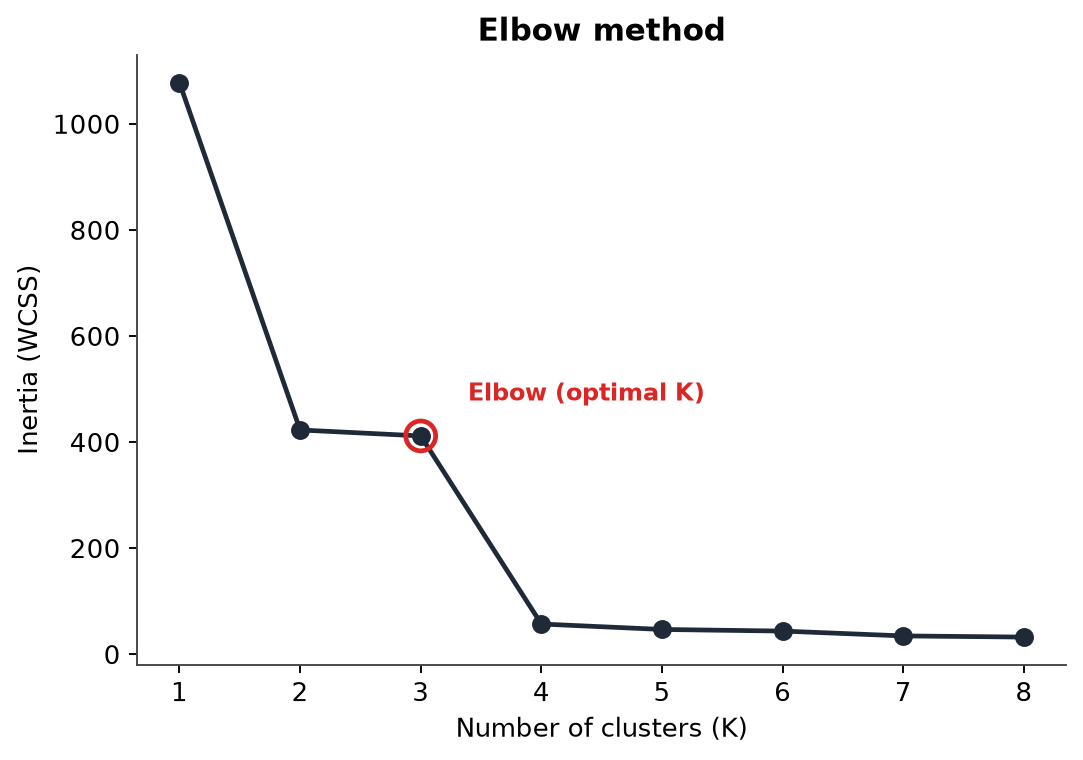
\includegraphics[width=0.5\textwidth]{../book/_static/generated/figures/en/elbow_method.png}
  \end{center}
\end{frame}

\begin{frame}{Hierarchical clustering: dendrogram}
  \begin{itemize}
    \item Builds a hierarchy of clusters without fixing $K$ in advance
    \item Cutting the dendrogram at a given height defines the number of clusters
  \end{itemize}
  \begin{center}
    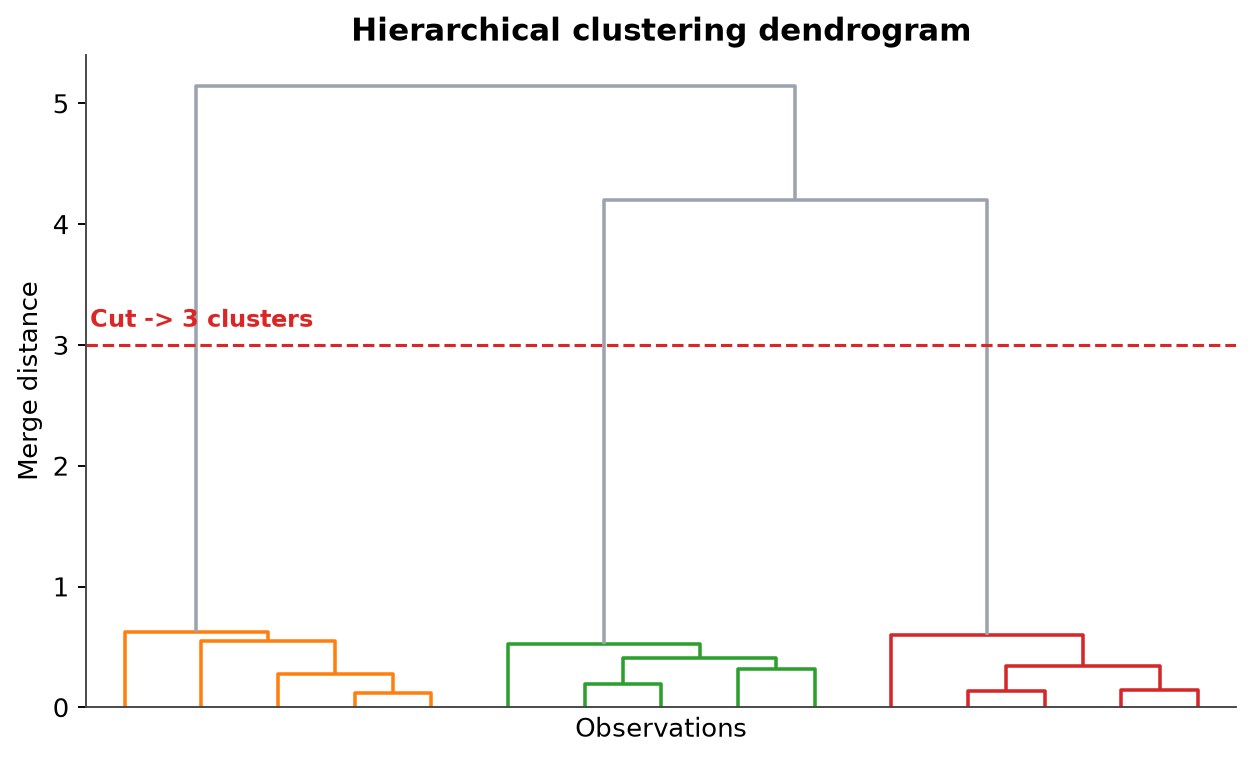
\includegraphics[width=0.6\textwidth]{../book/_static/generated/figures/en/dendrogram.png}
  \end{center}
\end{frame}

\begin{frame}{Real data: NCI60 (cancer cell lines)}
  \begin{columns}
    \begin{column}{0.45\textwidth}
      \begin{itemize}
        \item Groups cancer cell lines by gene-expression similarity
        \item Lines of the same cancer type tend to cluster on the same branch
      \end{itemize}
      \fuente{James, Witten, Hastie \& Tibshirani (2013), \textit{An Introduction to Statistical Learning}, Fig. 10.17.}
    \end{column}
    \begin{column}{0.4\textwidth}
      \centering
      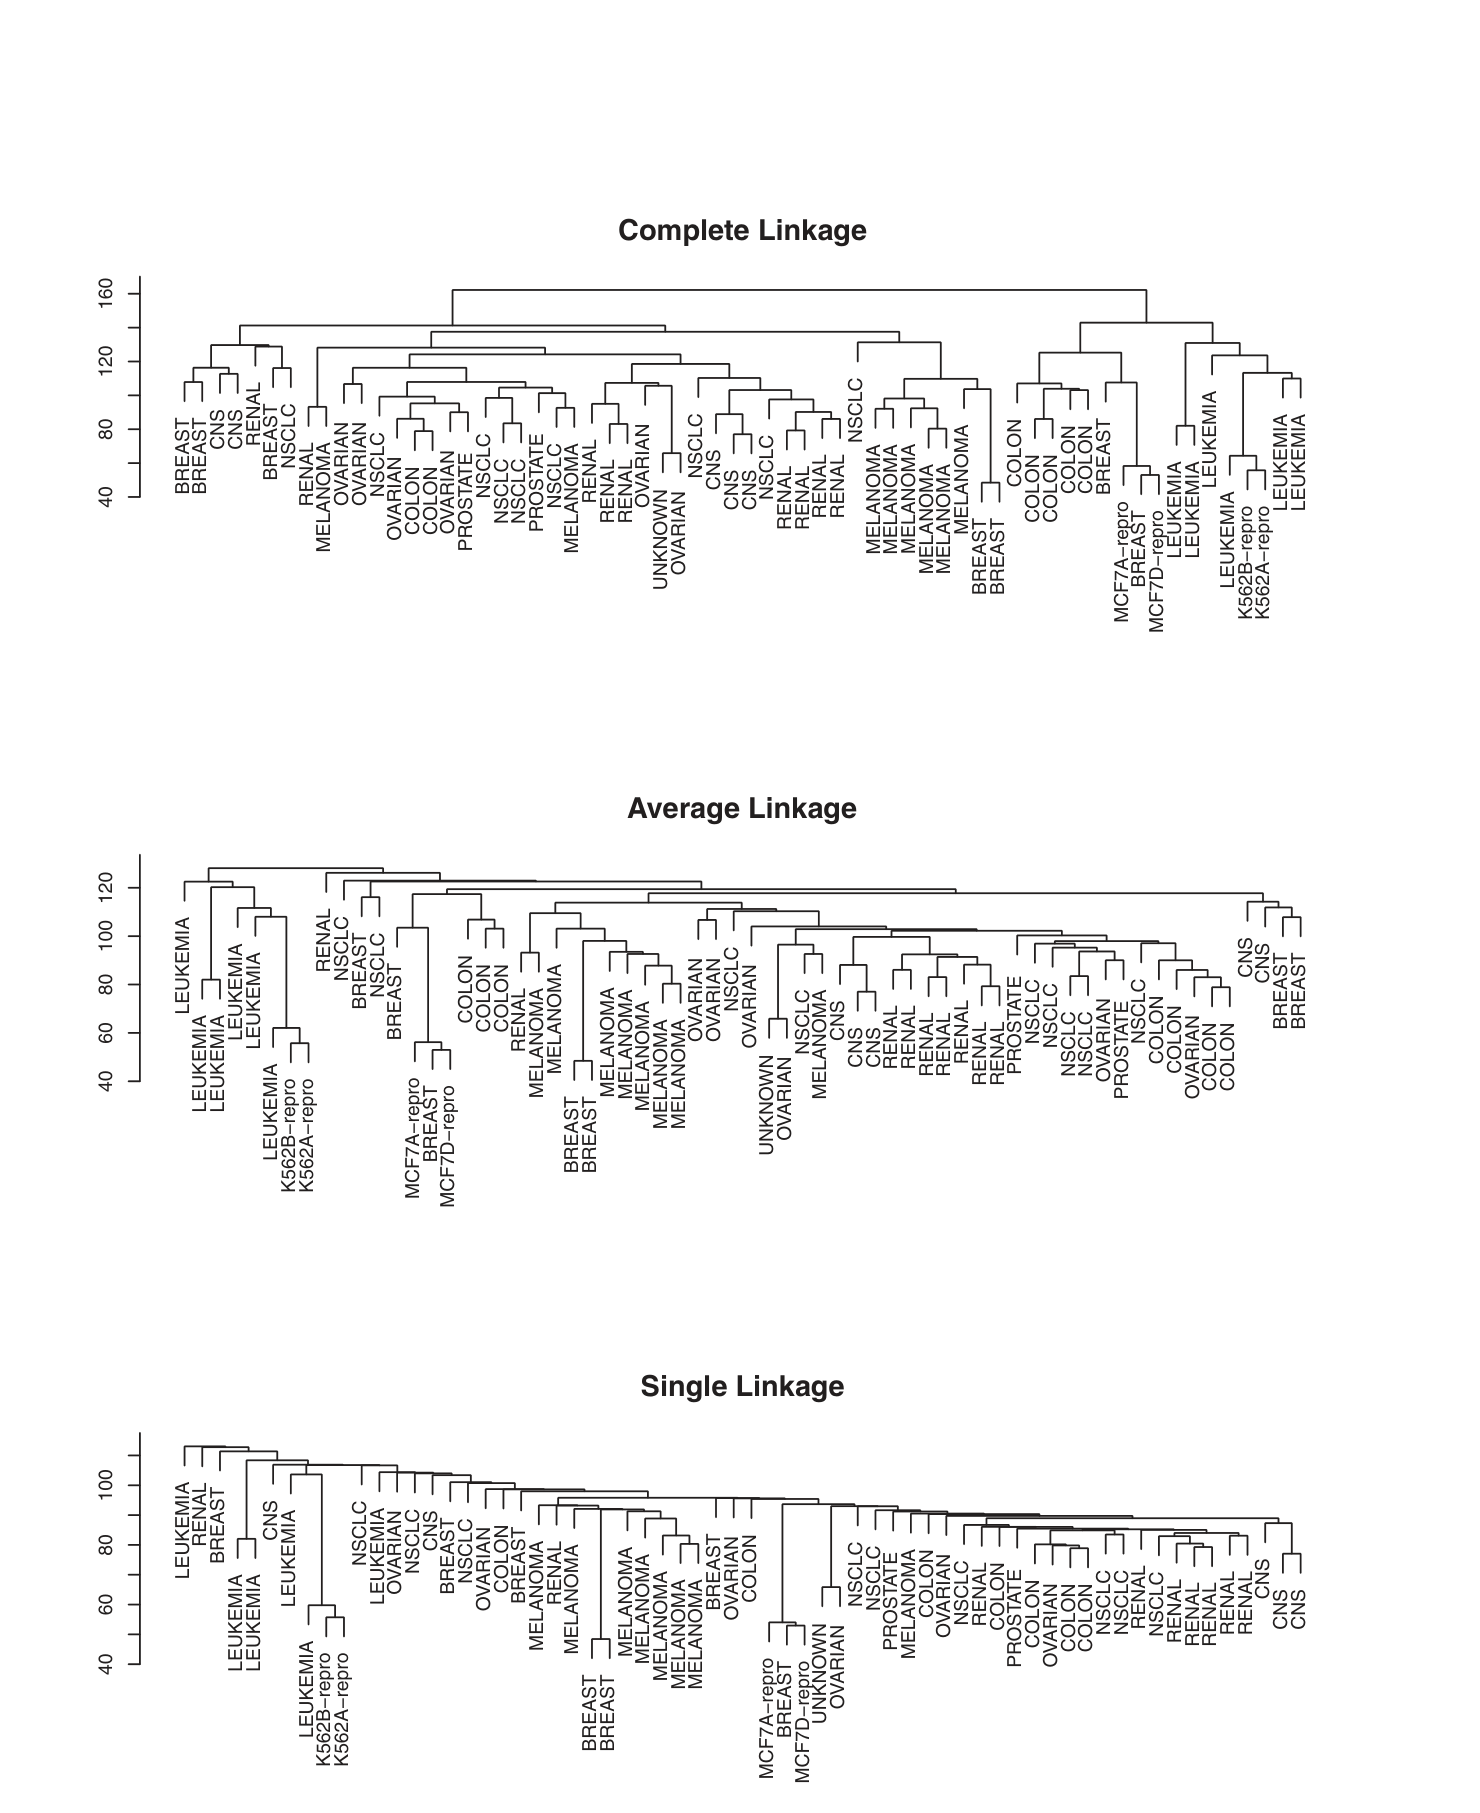
\includegraphics[width=\textwidth]{../book/_static/book_figures/islr_fig10_17_nci60_dendrogram.png}
    \end{column}
  \end{columns}
\end{frame}

\begin{frame}{DBSCAN vs. $K$-means}
  \footnotesize
  DBSCAN clusters by density: no need to fix $K$, it detects arbitrary shapes and automatically identifies noise (points belonging to no cluster).
  \begin{center}
    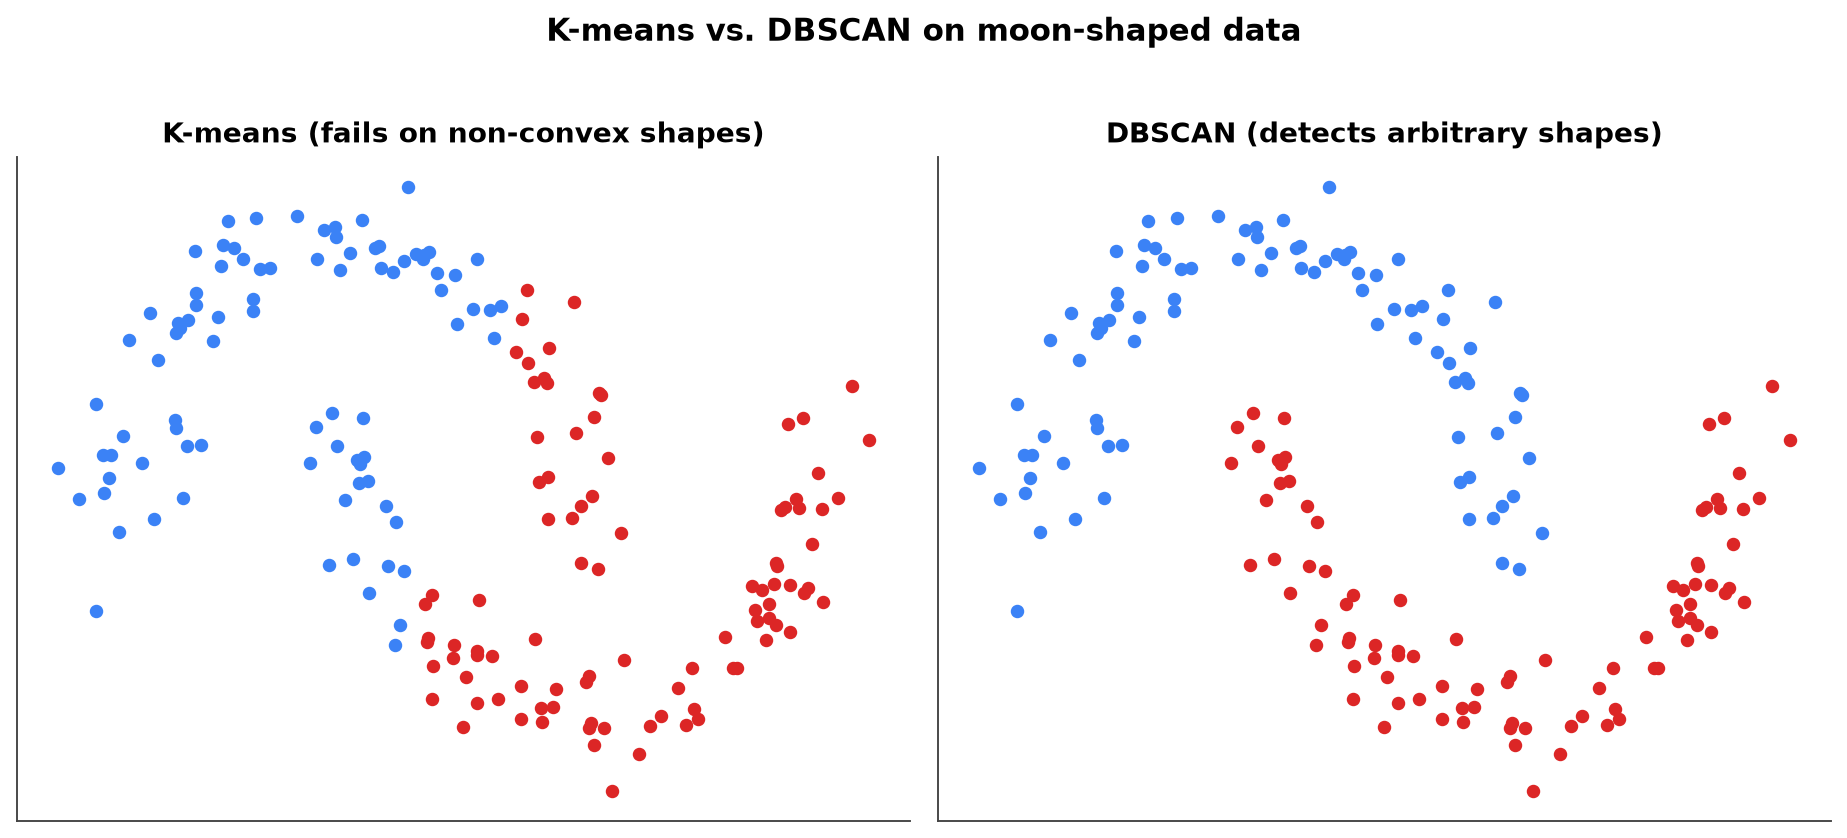
\includegraphics[width=0.85\textwidth]{../book/_static/generated/figures/en/dbscan_vs_kmeans.png}
  \end{center}
\end{frame}

\begin{frame}{Evaluation: silhouette coefficient}
  \begin{itemize}
    \item Measures how similar a point is to its own cluster versus others
    \item Range $[-1, 1]$: high values indicate well-separated clusters
  \end{itemize}
  \begin{center}
    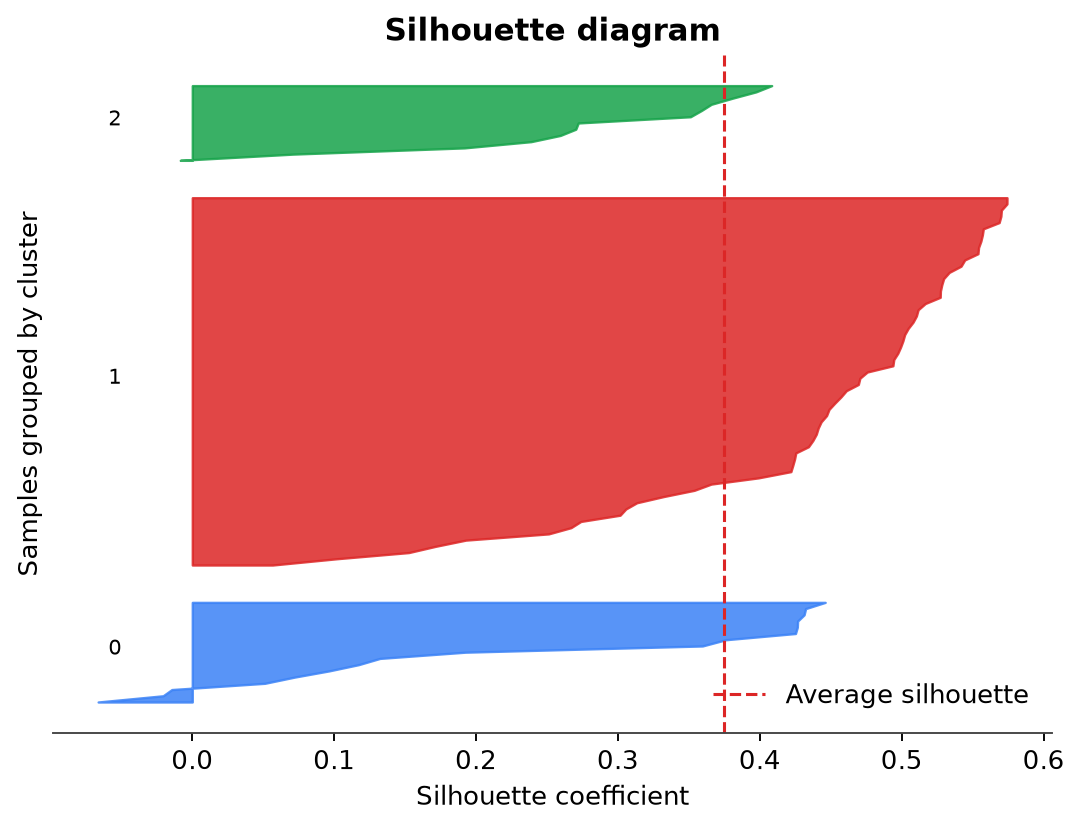
\includegraphics[width=0.45\textwidth]{../book/_static/generated/figures/en/silhouette_diagram.png}
  \end{center}
\end{frame}

\subsection{3.2 Dimensionality reduction}

\begin{frame}{The curse of dimensionality}
  \footnotesize
  As dimensions increase, data becomes extremely sparse and distances between points become nearly indistinguishable.
  \begin{center}
    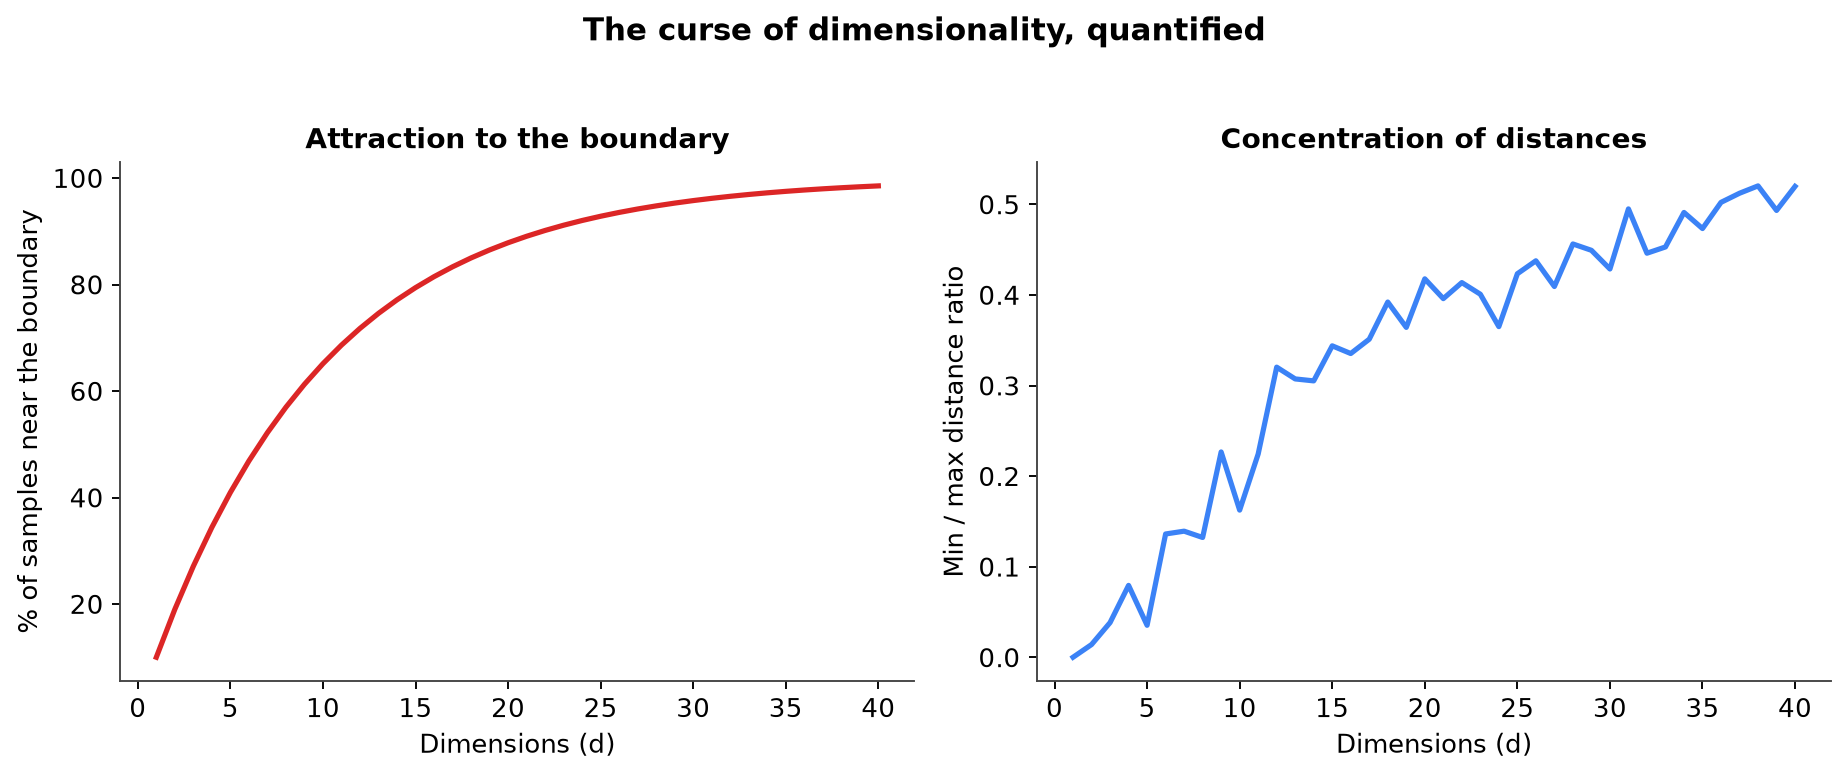
\includegraphics[width=0.85\textwidth]{../book/_static/generated/figures/en/curse_of_dimensionality.png}
  \end{center}
\end{frame}

\begin{frame}{PCA: principal components}
  \begin{itemize}
    \item PC1: direction of maximum variance; PC2: orthogonal, captures remaining variance
    \item Reduces dimensionality while preserving most of the information
  \end{itemize}
  \begin{center}
    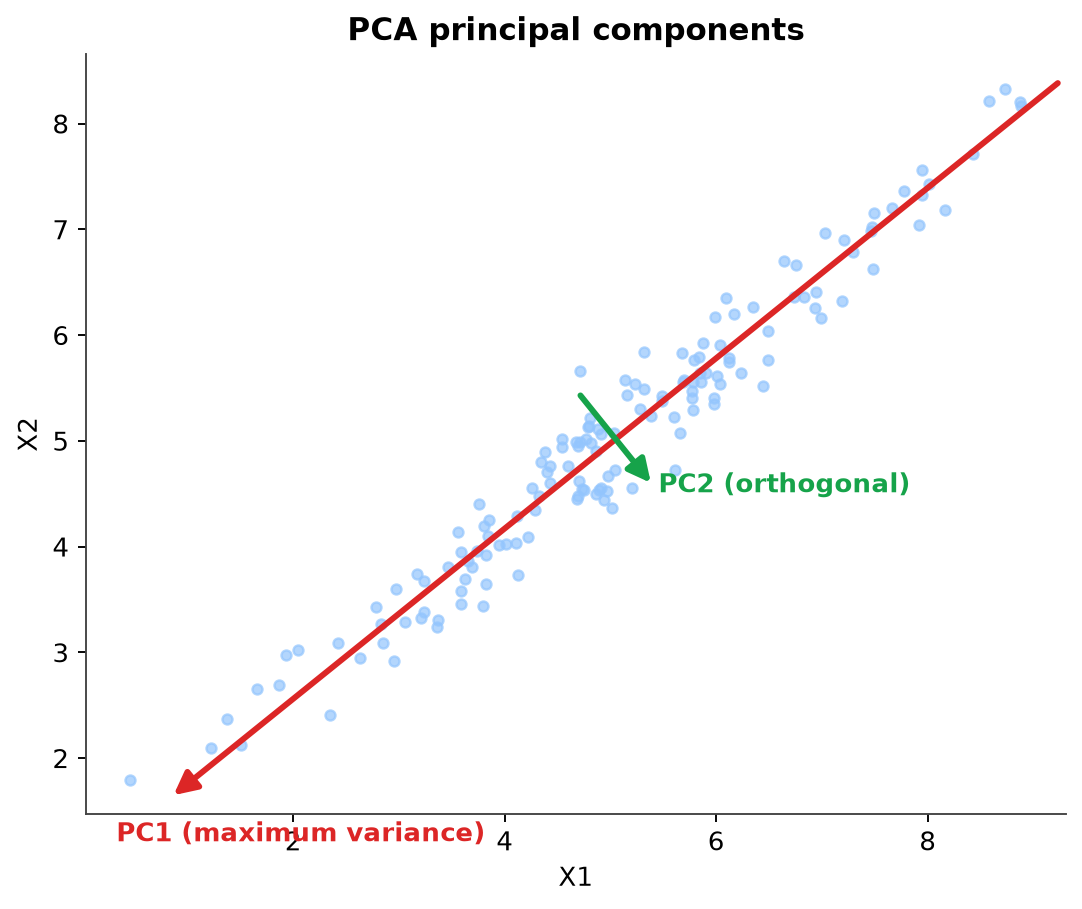
\includegraphics[width=0.45\textwidth]{../book/_static/generated/figures/en/pca_projection.png}
  \end{center}
\end{frame}

\begin{frame}{PCA on real data: NCI60 (6830 genes)}
  \footnotesize
  From 6830 genes down to just 3 principal components: lines of the same cancer type (same color) cluster together despite the huge original dimensionality.
  \begin{center}
    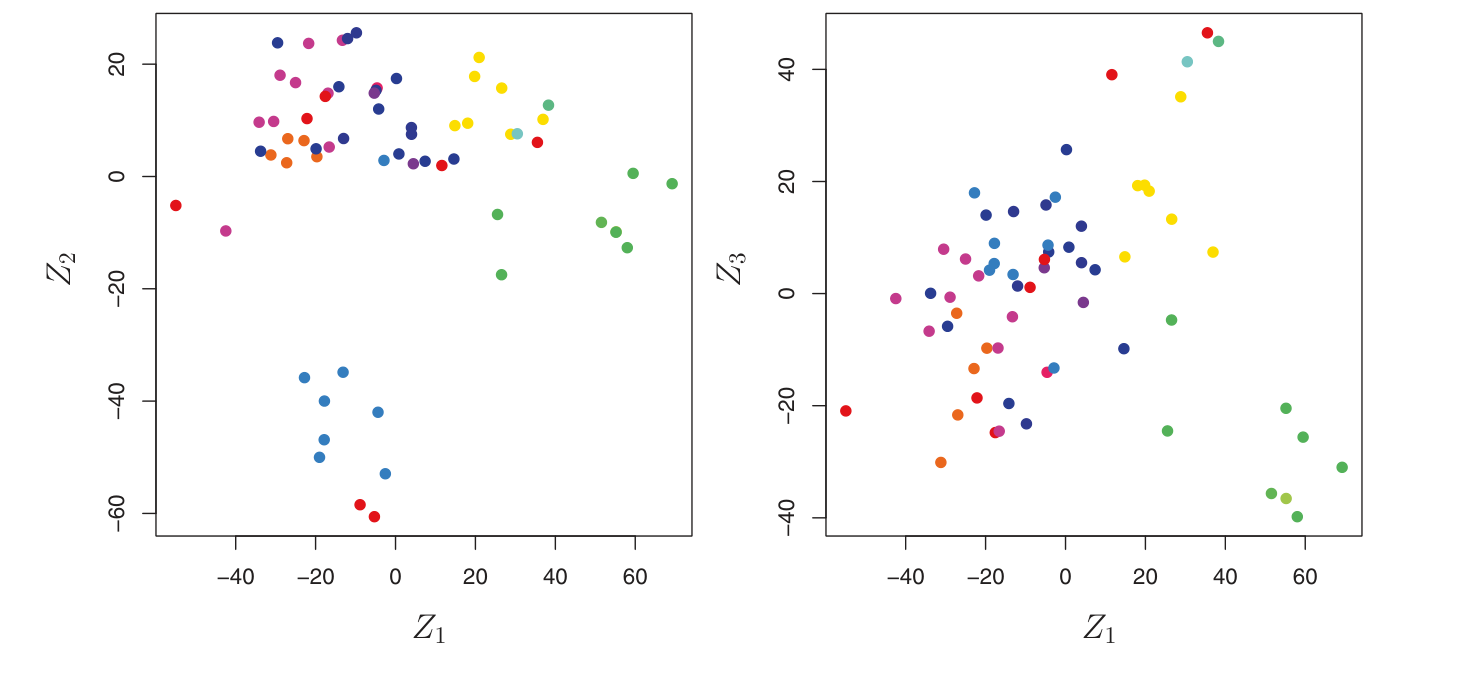
\includegraphics[width=0.65\textwidth]{../book/_static/book_figures/islr_fig10_15_nci60_pca.png}
  \end{center}
  \fuente{James, Witten, Hastie \& Tibshirani (2013), \textit{An Introduction to Statistical Learning}, Fig. 10.15.}
\end{frame}

\begin{frame}{\textit{Manifold learning}: the Swiss roll}
  \footnotesize
  Linear PCA would collapse distant points on the rolled-up surface; \textit{manifold learning} ``unrolls'' the surface while preserving local distances.
  \begin{center}
    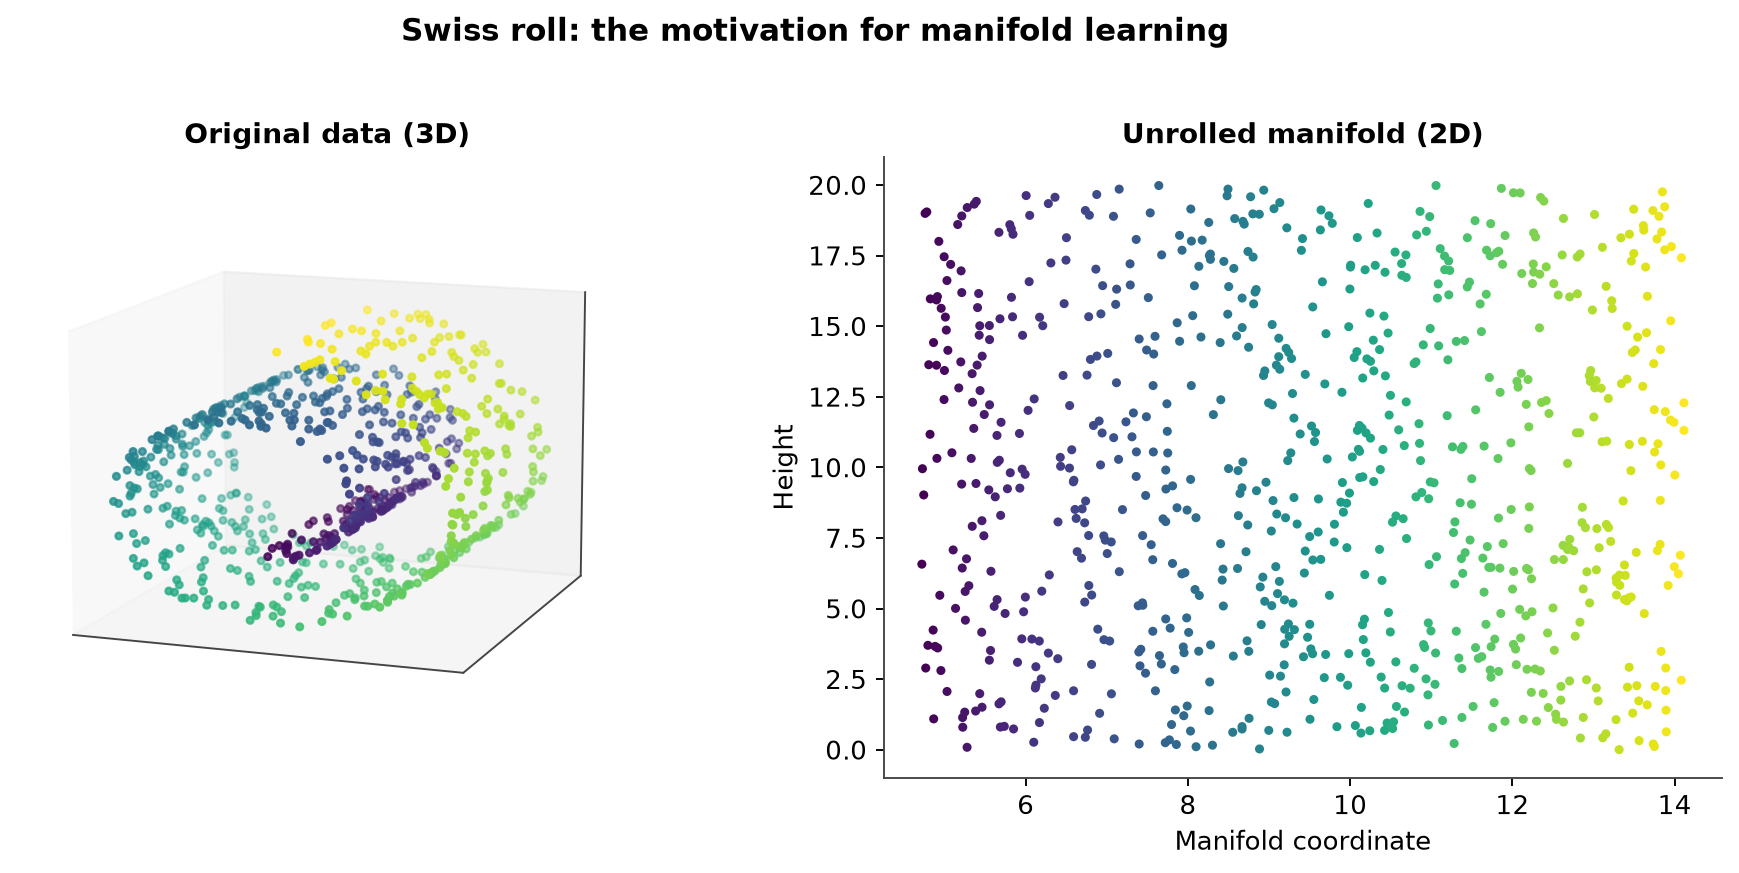
\includegraphics[width=0.85\textwidth]{../book/_static/generated/figures/en/swiss_roll_manifold.png}
  \end{center}
\end{frame}

\begin{frame}{t-SNE and UMAP}
  \begin{itemize}
    \item \textbf{t-SNE}: preserves local neighborhoods; excellent for visualization, slow on large datasets
    \item \textbf{UMAP}: faster, better preserves global structure
    \item Both are non-linear — they capture relationships PCA cannot
  \end{itemize}
\end{frame}

\subsection{3.3 Anomaly detection}

\begin{frame}{Philosophy of anomaly detection}
  \begin{itemize}
    \item \textit{Inliers} (normal) vs. \textit{outliers} (anomalies)
    \item \textbf{Anomaly detection}: contaminated training dataset
    \item \textbf{Novelty detection}: clean training dataset
  \end{itemize}
\end{frame}

\begin{frame}{Gaussian approach}
  \begin{itemize}
    \item Fits a (multivariate) Gaussian distribution to the normal data
    \item Points with low probability density are flagged as anomalies
  \end{itemize}
  \begin{center}
    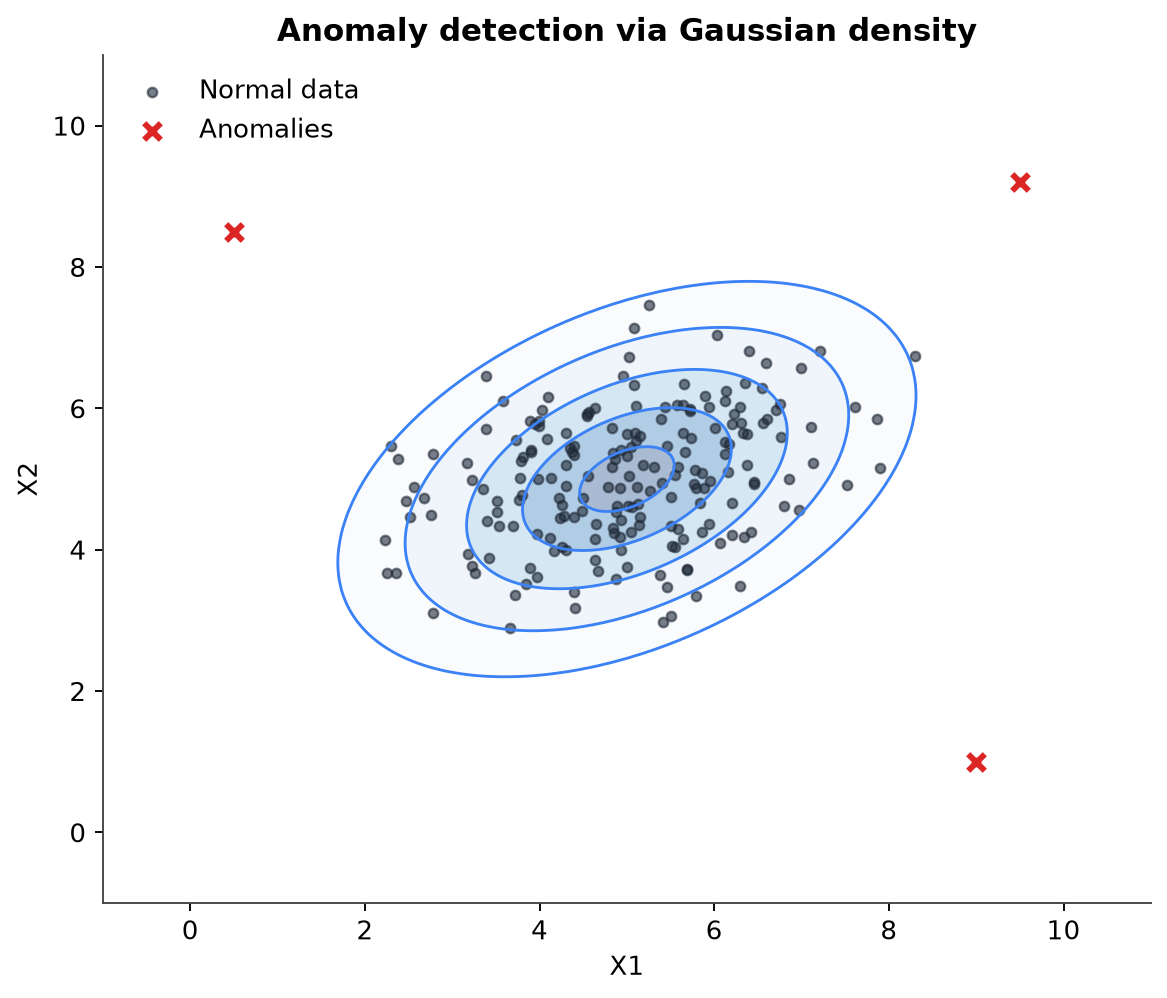
\includegraphics[width=0.42\textwidth]{../book/_static/generated/figures/en/gaussian_anomaly_detection.png}
  \end{center}
\end{frame}

\begin{frame}{Isolation Forest}
  \footnotesize
  Isolates points via random partitions of the feature space: anomalies require very few partitions to become isolated.
  \begin{center}
    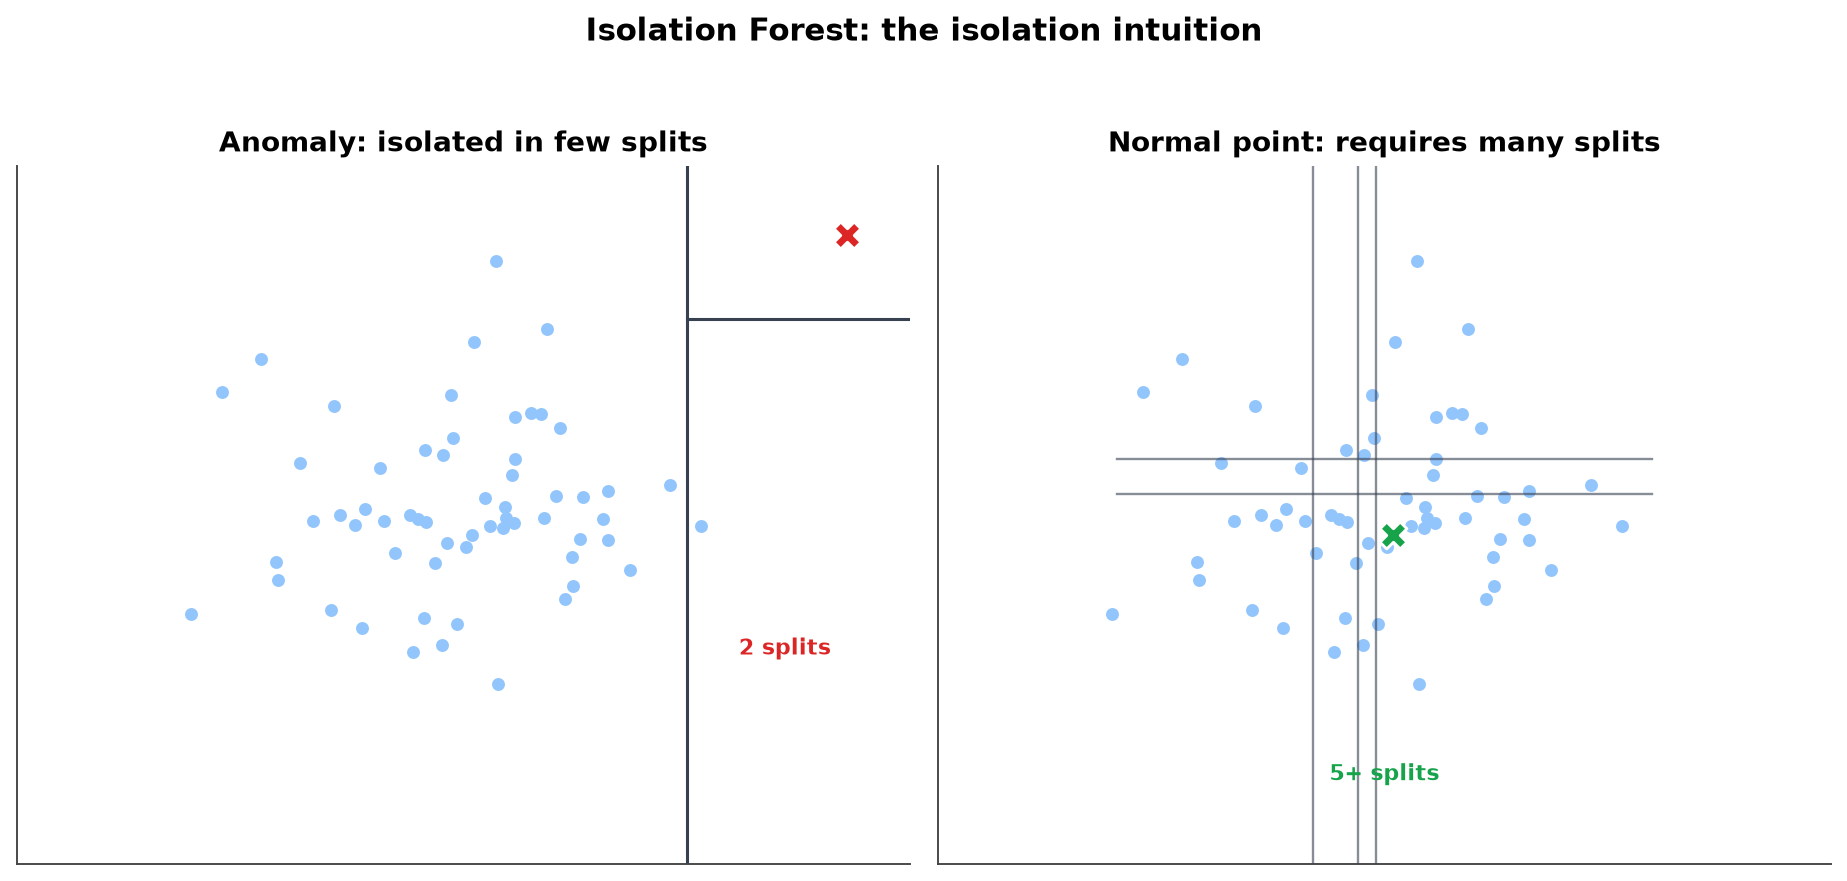
\includegraphics[width=0.85\textwidth]{../book/_static/generated/figures/en/isolation_forest_concept.png}
  \end{center}
\end{frame}

\begin{frame}{Local Outlier Factor (LOF)}
  \begin{itemize}
    \item Compares a point's local density with that of its neighbors
    \item Detects local anomalies that a global density threshold would miss
  \end{itemize}
  \begin{center}
    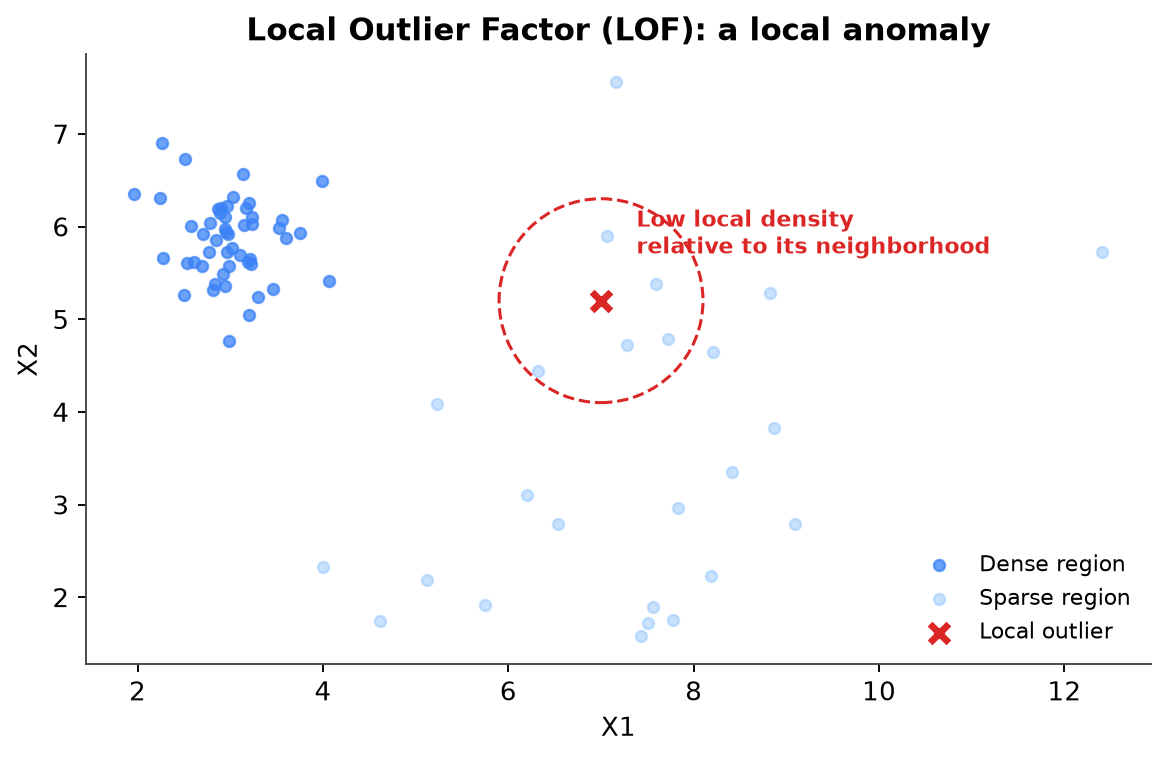
\includegraphics[width=0.42\textwidth]{../book/_static/generated/figures/en/lof_concept.png}
  \end{center}
\end{frame}

% ============================================================
\begin{frame}{Course summary}
  \begin{columns}
    \begin{column}{0.33\textwidth}
      \textbf{Foundations}
      \begin{itemize}
        \footnotesize
        \item History of ML
        \item Overfitting/underfitting
        \item Cross-validation
      \end{itemize}
    \end{column}
    \begin{column}{0.33\textwidth}
      \textbf{Supervised}
      \begin{itemize}
        \footnotesize
        \item Regression, regularization
        \item Classification, SVM
        \item Neural networks
      \end{itemize}
    \end{column}
    \begin{column}{0.33\textwidth}
      \textbf{Unsupervised}
      \begin{itemize}
        \footnotesize
        \item Clustering
        \item PCA, manifold learning
        \item Anomaly detection
      \end{itemize}
    \end{column}
  \end{columns}
\end{frame}

\begin{frame}
  \centering
  {\Huge Thank you!}\\[1em]
  {\large Universidad de Salamanca}
\end{frame}

\end{document}
